\section{Modèles non-linéaires à changement de régimes markoviens et asymétriques}

\begin{sloppypar}
Ce paragraphe présente les fondements théoriques des modèles économétriques avancés appliqués à l’analyse des interactions entre trois sous-indicateurs du CISS étudiés.\\

Le premier sous-paragraphe commence par une introduction aux chaînes de Markov. Les chaînes de Markov, initialement introduites par Andrey Markov en 1906, ont été développées pour étudier les dépendances entre événements dans des processus aléatoires. Markov a appliqué cette théorie à des séquences de lettres dans des textes littéraires, démontrant ainsi qu'il est possible de modéliser des systèmes où l'état futur dépend uniquement de l'état présent, et non de l'ensemble des états passés. Depuis lors, ces chaînes sont devenues un outil très utilisé en mathématiques appliquées, économie et physique, pour modéliser des phénomènes de changements de régimes.\\

Le second sous-paragraphe approfondit la spécification du modèle Markov Switching-VAR en expliquant ses typologies et les méthodologies associées, telles que la décomposition de Cholesky, les moments conditionnels et les réponses aux chocs. Les typologies incluent des modèles à variances constantes ou variables selon les régimes, tandis que les moments conditionnels permettent d’étudier la dynamique des réponses des variables aux chocs exogènes dans chaque régime. La décomposition de Cholesky est utilisée pour identifier les chocs structurels dans les séries temporelles.
Enfin, dans ce sous-paragraphe, il est présenté les méthodes d'estimation et de filtrage avec l'algorithme de Hamilton pour illustrer l’ajustement des modèles dans un cadre multirégime. Cet algorithme est crucial pour estimer les probabilités ex-post des régimes et les paramètres du modèle, en maximisant la vraisemblance jointe des observations dans un cadre non-linéaire.\\

Le dernier sous-paragraphe introduit le modèle univarié NARDL pour analyser les dynamiques non-linéaires asymétriques. Ce modèle permet de capturer les effets asymétriques des variations positives et négatives d’une variable explicative sur une variable dépendante. Il est particulièrement adapté pour analyser des phénomènes économiques où les ajustements aux chocs diffèrent selon leur direction, offrant ainsi une perspective complémentaire au MS-VAR dans le cadre des sous-indicateurs du CISS.

\subsection{Chaîne de Markov}

Les chaînes de Markov offrent un cadre mathématique pour modéliser les processus stochastiques où l’évolution d’un système est latent. En économétrie, ce concept se révèle particulièrement utile pour décrire des phénomènes économiques présentant des changements d’état abrupts ou des transitions entre différents régimes. Ce sous-paragraphe introduit les chaînes de Markov en explorant leurs caractéristiques fondamentales, telles que la relation de Chapman-Kolmogorov, qui exprime la probabilité de transition entre états sur plusieurs étapes, ainsi que la classification des états, qui permet de distinguer entre les états récurrents et transients. La périodicité et les lois de probabilité stationnaires viennent compléter cette étude, fournissant ainsi les bases nécessaires pour appliquer les chaînes de Markov dans des modèles utilisés lors de ce projet qui est le modèle Markov Switching-VAR.

\subsubsection{Généralités sur les chaînes de Markov}
Afin d'illustrer cette partie, la présentation de la notion de Chaînes de Markov est amplement tirée du cours de préparation à l'agrégation de mathématiques de l'Université de Bordeaux 1 de \cite[2013]{Ruch et Chabanol}.\\

Les chaînes de Markov constituent un des exemples les plus simples de suites de variables aléatoires $(X_n)$. 
Les variables $(X_n)$ sont à valeurs dans un ensemble $E$ appelé espace d’état. 
Certaines chaînes de Markov sont à espace d’états continu, mais il ne sera pas abordé leur étude ici. 
Seules les chaînes à espace d’états fini ou dénombrable. 
Dans toute la suite, $E$ sera donc un ensemble fini ou dénombrable ($\mathbb{N}$ ou un sous-ensemble), que l’on munira de la tribu de toutes ses parties. 

\begin{tcolorbox}[colback=blue!5!white,colframe=blue!75!black,title=Définition]
Une suite $(X_n)_{n \geq 0}$ de variables aléatoires à valeurs dans un ensemble au plus dénombrable $E$ est une chaîne de Markov d’espace d’états $E$ si et seulement si pour tout $k \in \mathbb{N}$,
pour tout $(x_0,...,x_{k+1})$ dans $E$ tels que $\mathbb{P}(X_k = x_k,...,X_0 = x_0) > 0$,

\begin{equation}
\mathbb{P}(X_{k+1} = x_{k+1} \mid X_k = x_k,...,X_0 = x_0) = \mathbb{P}(X_{k+1} = x_{k+1} \mid X_k = x_k).    
\end{equation}

Cela s’écrit également

\begin{equation}
\mathcal{L}(X_{k+1} \mid X_k = x_k,...,X_0 = x_0) = \mathcal{L}(X_{k+1} \mid X_k = x_k)    
\end{equation}

pour tout $k \in \mathbb{N}$.\\

Cela signifie que seule la valeur de l'état actuel \(X_t\) influe sur la probabilité de l'état futur \(X_{t+1}\).\\
\end{tcolorbox}


La chaîne est dite homogène si il y a de plus pour tout $k \in \mathbb{N}$ et tout $x$ et $y$ dans $E$,
\begin{equation}
    \mathbb{P}(X_{k+1} = y \mid X_k = x) = \mathbb{P}(X_1 = y \mid X_0 = x)  
\end{equation}

\begin{tcolorbox}[colback=blue!5!white,colframe=blue!75!black,title=Définition]
    On appelle probabilité de transition pour aller de l’état $x$ à l’état $y$ la probabilité
    \begin{equation}
    p_{x,y} = \mathbb{P}(X_{k+1} = y \mid X_k = x) (= \mathbb{P}(X_1 = y \mid X_0 = x)).
    \end{equation}
    \end{tcolorbox}


Il est noté $\nu_0$ la loi de $X_0$ ($\nu_0(x_0) = \mathbb{P}(X_0 = x_0)$). Il est donc obtenu que pour tout $(x_0, \dots, x_n) \in E$

\begin{equation}
\mathbb{P}(X_n = x_n, \dots, X_0 = x_0) = \nu_0(x_0) \prod_{k=0}^{n-1} p_{x_k, x_{k+1}}.   
\end{equation}

En effet, 
\begin{equation}
\begin{split}
 &\mathbb{P}(X_n = x_n, \dots, X_0 = x_0) = \mathbb{P}(X_0 = x_0) \mathbb{P}(X_1 = x_1 \mid X_0 = x_0) \\
&\mathbb{P}(X_2 = x_2 \mid X_1 = x_1, X_0 = x_0) \dots \mathbb{P}(X_n = x_n \mid X_{n-1} = x_{n-1}, \dots, X_0 = x_0)\\
&= \nu(x_0) \prod_{k=0}^{n-1} p_{x_k, x_{k+1}}.
\end{split}   
\end{equation}

\begin{tcolorbox}[colback=blue!5!white,colframe=blue!75!black,title=Définition]
Il est appellé matrice de transition la matrice $\mathcal{P} = (p_{x,y})_{x,y \in E}$ :
\begin{equation}
\mathcal{P} =
\begin{pmatrix}
p_{x_0,x_0} & p_{x_0,x_1} & p_{x_0,x_2} & \cdots \\
p_{x_1,x_0} & p_{x_1,x_1} & p_{x_1,x_2} & \cdots \\
p_{x_2,x_0} & p_{x_2,x_1} & p_{x_2,x_2} & \cdots \\
\vdots & \vdots & \vdots & \ddots
\end{pmatrix}.   
\end{equation}

D'après le lemme précédent, la loi d'une chaîne de Markov est caractérisée par la loi $\nu_0$ de $X_0$ et par
sa matrice de transition.
\end{tcolorbox}

Toute matrice de transition vérifie les propriétés suivantes dérivées des définitions probabilistes :
\begin{enumerate}
    \item Pour tout couple $(x,y) \in E$, $0 \leq p_{x,y} \leq 1$ ;
    \item Pour tout $x \in E$, on a $\sum_{y \in E} p_{x,y} = 1$.
\end{enumerate}

\begin{tcolorbox}[colback=green!5!white,colframe=green!75!black,title=Proposition]
Il est identifié une probabilité $\mu$ sur $E$ et le vecteur ligne dont la $i$-ème coordonnée est
$\mu(x_i)$. Soit $(X_n)$ une chaîne de Markov de matrice de transition $P$, et soit $\nu_0$ la loi de $X_0$. Alors la loi de
$X_1$ est $\nu_1 = \nu_0 \mathcal{P}$, et pour tout entier $n$, la loi de $X_n$ est $\nu_n = \nu_0 \mathcal{P}^n$.
\end{tcolorbox}

Pour le premier point, il est établi pour tout $x_i \in E$,

\begin{equation}
\mathbb{P}(X_1 = x_i) = \sum_{x_j \in E} \mathbb{P}(X_1 = x_i \mid X_0 = x_j) \mathbb{P}(X_0 = x_j) = \sum_{x_j \in E} \nu_0(x_j) \mathcal{P}_{j,i} = (\nu_0 \mathcal{P})_i.   
\end{equation}

(en posant par convention $P(A \mid B) P(B) = 0$ si $P(B) = 0$). 
Ensuite,  il peut être procédé par récurrence. Il est à noter $(Q_n)$ la proposition $\nu_n = \nu_0 \mathcal{P}^n$. Il vient d'être prouver $Q_1$. Il reste à vérifier l’hérédité. Soit $n > 0$. Il est supposé $\nu_n = \nu_0 \mathcal{P}^n$. Alors pour tout $x_i \in E$,

\begin{equation}
   \mathbb{P}(X_{n+1} = x_i) = \sum_{x_j \in E} \mathbb{P}(X_{n+1} = x_i \mid X_n = x_j) \mathbb{P}(X_n = x_j) = \sum_{x_j \in E} \nu_n(j) \mathcal{P}_{j,i} = (\nu_0 \mathcal{P}^{n+1})_i 
\end{equation}

Ainsi, l'évolution de la loi de $X_n$ se ramène en fait à de l'algèbre linéaire. À toute matrice de transition, un graphe dirigé peut être associé, éventuellement infini. Les sommets du
graphe sont les différents états de la chaîne. Il y a une flèche, étiquetée $p_{x,y}$, entre le sommet $x$ et le
sommet $y$ si et seulement si la probabilité de transition est strictement positive : $p_{x,y} > 0$. La chaîne peut
alors s’interpréter comme une marche aléatoire sur le graphe. Cela donne par exemple pour trois régimes : 

\begin{center}
\begin{tikzpicture}[->, >=stealth', auto, semithick, node distance=4cm]

    \tikzstyle{state}=[circle,thick,draw=black,fill=gray!10,minimum size=2cm]
  
    % Nodes
    \node[state] (R1) {Régime 1};
    \node[state] (R2) [right of=R1] {Régime 2};
    \node[state] (R3) [below of=R1, xshift=2cm, yshift=-1cm] {Régime 3};
  
    % Edges
    \path (R1) edge [loop left] node{\(p_{11}\)} (R1)
              edge [bend left=20] node{\(p_{12}\)} (R2)
              edge [bend right=20] node[below left]{\(p_{13}\)} (R3)
          (R2) edge [loop right] node{\(p_{22}\)} (R2)
              edge [bend left=20] node{\(p_{21}\)} (R1)
              edge [bend left=20] node[below right]{\(p_{23}\)} (R3)
          (R3) edge [loop below] node{\(p_{33}\)} (R3)
              edge [bend right=25] node[above left]{\(p_{31}\)} (R1)
              edge [bend left=27] node[above right]{\(p_{32}\)} (R2);
  
  \end{tikzpicture}
\end{center}

\subsubsection{Relation de Chapman-Kolmogorov}

Ainsi, est appelée la propriété reliant, pour une chaîne de Markov homogène, les probabilités de transition
en $n$ étapes aux probabilités en une seule étape.\\

Il est à noter $(X_n)_{n \geq 0}$ une chaîne de Markov homogène, dont l’ensemble des états est $E$ et la matrice de transition $\mathcal{P} = (p_{i,j})_{(i,j) \in E^2}$. Pour $n \geq 0$ et $i, j \in E$, il est désigné par $p^{(n)}_{i,j}$ la probabilité, partant de l’état $i$
à l’instant $0$, d’être dans l’état $j$ à l’instant $n$; en d’autres termes on a :

\begin{equation}
 p^{(n)}_{i,j} = \mathbb{P}(X_n = j \mid X_0 = i)   
\end{equation}

La relation de Chapman-Kolmogorov qui suit peut s’interpréter en disant que “pour passer de $i$ à $j$ en
$m + n$ étapes, il a bien fallu en $m$ étapes aller de $i$ à un certain $k$, puis en $n$ étapes aller de $k$ à $j$.

\begin{tcolorbox}[colback=green!5!white,colframe=green!75!black,title=Proposition]
Pour tout $(i, j) \in E^2$ et tout couple $(m, n)$ d’entiers positifs, on a l’identité :
    
\begin{equation}
 \mathbb{P}(X_{m+n} = j \mid X_0 = i) = \sum_{k \in E} \mathbb{P}(X_m = k \mid X_0 = i) \, \mathbb{P}(X_n = j \mid X_0 = k)   
\end{equation}
    
ou encore
    
\begin{equation}
  p^{(m+n)}_{i,j} = \sum_{k \in E} p^{(m)}_{i,k} \, p^{(n)}_{k,j}
\end{equation}
\end{tcolorbox}

Cette identité résulte immédiatement de l’associativité du produit matriciel :

\begin{equation}
 \mathcal{P}^{(m+n)} = \mathcal{P}^{m+n} = \mathcal{P}^m \mathcal{P}^n = \mathcal{P}^{(m)} \mathcal{P}^{(n)}   
\end{equation}

\subsubsection{Classification des états d'une chaîne markovienne}

Une classification des états va être définie, et des propriétés des chaînes de Markov en seront déduites. Les 
états d’une chaîne de Markov sont répartis en classes, définies à partir de la matrice de transition.

\begin{tcolorbox}[colback=blue!5!white,colframe=blue!75!black,title=Définition]
L’état $j$ est dit \emph{accessible} à partir de l’état $i$, s’il existe un entier $n \geq 0$ tel que $p^{(n)}_{i,j} > 0$. On note $i \rightarrow j$. Sur le graphe, si $i \neq j$, $i \rightarrow j$ s’il existe un chemin (orienté) du sommet $i$ vers le sommet $j$. La relation d’accessibilité entre états est réflexive\footnote{Dans le contexte d'une chaîne de Markov, une relation réflexive signifie qu'un état est accessible à partir de lui-même.} et transitive.
\end{tcolorbox}

Comme $p^{(0)}_{i,i} = \mathbb{P}(X_0 = i \mid X_0 = i) = 1$ pour tout état $i$, la relation est réflexive. Ensuite, si $i \rightarrow j$ et $j \rightarrow l$, alors $p^{(m)}_{i,j} > 0$ et $p^{(n)}_{j,l} > 0$ pour certains entiers $m, n \geq 0$.\\

D'après la relation de Chapman-Kolmogorov, on a :

\begin{equation}
 \mathbb{P}(X_{m+n} = l \mid X_0 = i) = \sum_{k \in E} \mathbb{P}(X_m = k \mid X_0 = i) \mathbb{P}(X_n = l \mid X_0 = k) \geq p^{(m)}_{i,j} p^{(n)}_{j,l} > 0   
\end{equation}

d'où $i \rightarrow l$.\\

Soient $i, j$ deux états; les deux propriétés suivantes sont équivalentes :

\begin{enumerate}
    \item[(a)] l’état $j$ est accessible à partir de l’état $i$, soit $i \rightarrow j$.
    \item[(b)] le processus, partant de $i$, passe par $j$ avec probabilité strictement positive.
\end{enumerate}

D'abord, $(a) \Rightarrow (b)$ est évident. Pour l’autre implication, montrons $(\neg a) \Rightarrow (\neg b)$. Il en résulte donc que, pour tout $n \geq 0$, $p^{(n)}_{i,j} = 0$. Soit $A$ l’événement “le processus passe par $j$”. On a

\begin{equation}
  \mathbb{P}(A \mid X_0 = i) = \mathbb{P}\left(\bigcup_{n \geq 0} \{X_n = j\} \mid X_0 = i\right) \leq \sum_{n \geq 0} \mathbb{P}(X_n = j \mid X_0 = i) = \sum_{n \geq 0} p^{(n)}_{i,j} = 0.  
\end{equation}

d'où la propriété $(b)$.

\begin{tcolorbox}[colback=blue!5!white,colframe=blue!75!black,title=Définition]
Il est dit que les états $i$ et $j$ \emph{communiquent} et on écrit $i \leftrightarrow j$ si on a à la fois $i \rightarrow j$ et $j \rightarrow i$. La relation de "communication" est une relation d’équivalence.
\end{tcolorbox}

Comme il est toujours vrai que $p^{(0)}_{i,i} = 1$, tout état communique avec lui-même.\\

Les classes\footnote{Dans le contexte des chaînes de Markov, une classe est un groupe d’états qui partagent une relation d’accessibilité. Plus précisément, une classe est un ensemble d'états tels que chacun de ces états peut être atteint à partir de n'importe quel autre état dans ce même ensemble, et vice-versa.} d'équivalence de cette relation sont les composantes fortement connexes du graphe. 
Appelé souvent \emph{composantes irréductibles} ou \emph{classes irréductibles}.\\

\begin{center}
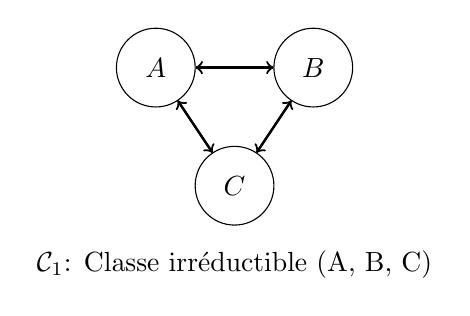
\begin{tikzpicture}
    % Définition des nœuds de la classe irréductible C1
    \node[circle, draw, minimum size=1cm] (A) at (0, 1.5) {$A$};
    \node[circle, draw, minimum size=1cm] (B) at (2, 1.5) {$B$};
    \node[circle, draw, minimum size=1cm] (C) at (1, 0) {$C$};

    % Arêtes internes à la classe irréductible C1
    \draw[->, thick] (A) -- (B) node[midway, above] {};
    \draw[->, thick] (B) -- (C) node[midway, right] {};
    \draw[->, thick] (C) -- (A) node[midway, left] {};
    
    % Boucles pour la communication bidirectionnelle
    \draw[->, thick] (B) -- (A) node[midway, below] {};
    \draw[->, thick] (C) -- (B) node[midway, left] {};
    \draw[->, thick] (A) -- (C) node[midway, right] {};

    % Légende des classes
    \node at (1, -1) {$\mathcal{C}_1$: Classe irréductible (A, B, C)};

\end{tikzpicture}
\end{center}


Si $\mathcal{C}_1$ et $\mathcal{C}_2$ étant deux classes distinctes, il est éventuellement possible d’aller, disons de $\mathcal{C}_1$ à $\mathcal{C}_2$, mais il est impossible de
retourner de $\mathcal{C}_2$ à $\mathcal{C}_1$. En revanche, tous les états d’une même classe communiquent.\\

\begin{center}
    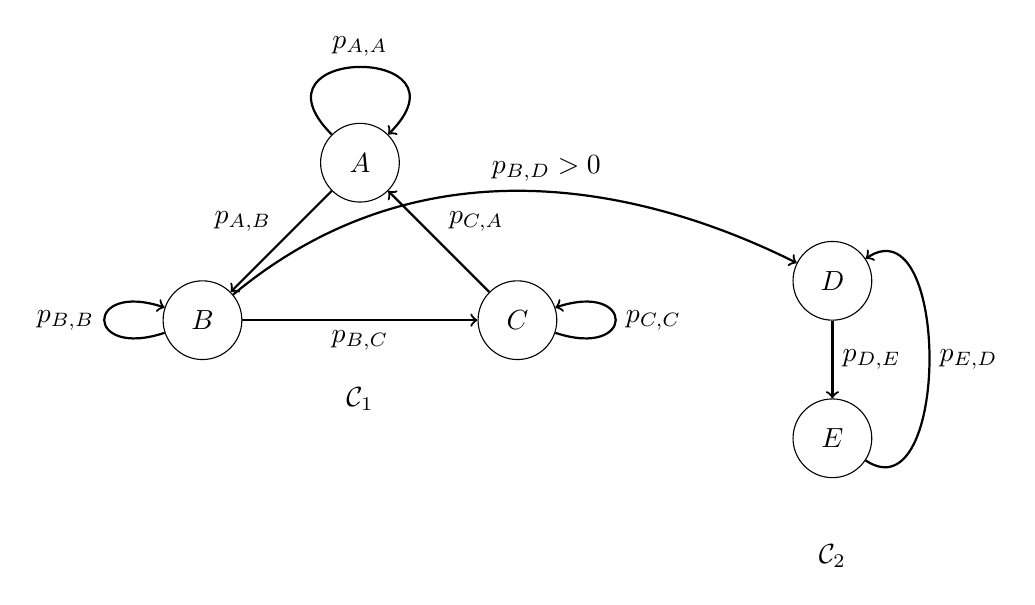
\begin{tikzpicture}
        % Définition des nœuds de la classe C1 en triangle et rehaussée
        \node[circle, draw, minimum size=1cm] (A1) at (0, 3) {$A$};
        \node[circle, draw, minimum size=1cm] (B1) at (-2, 1) {$B$};
        \node[circle, draw, minimum size=1cm] (C1) at (2, 1) {$C$};
        
        % Définition des nœuds de la classe C2 avec plus d'espace
        \node[circle, draw, minimum size=1cm] (D2) at (6, 1.5) {$D$};
        \node[circle, draw, minimum size=1cm] (E2) at (6, -0.5) {$E$};
    
        % Arêtes internes à la classe C1
        \draw[->, thick] (A1) -- (B1) node[midway, above left] {$p_{A,B}$};
        \draw[->, thick] (B1) -- (C1) node[midway, below] {$p_{B,C}$};
        \draw[->, thick] (C1) -- (A1) node[midway, above right] {$p_{C,A}$};
    
        % Boucles sur les nœuds de C1
        \draw[->, thick] (A1) .. controls (-1.5, 4.5) and (1.5, 4.5) .. (A1) node[midway, above] {$p_{A,A}$};
        \draw[->, thick] (B1) .. controls (-3.5, 0.5) and (-3.5, 1.5) .. (B1) node[midway, left] {$p_{B,B}$};
        \draw[->, thick] (C1) .. controls (3.5, 0.5) and (3.5, 1.5) .. (C1) node[midway, right] {$p_{C,C}$};
        
        % Arêtes internes à la classe C2
        \draw[->, thick] (D2) -- (E2) node[midway, right] {$p_{D,E}$};
        \draw[->, thick] (E2) .. controls (7.5, -1.5) and (7.5, 2.5) .. (D2) node[midway, right] {$p_{E,D}$};
    
        % Transition de C1 à C2 (réhaussée pour éviter de couper le graphe)
        \draw[->, thick] (B1) .. controls (1, 3.5) and (4, 2.5) .. (D2) node[midway, above] {$p_{B,D} > 0$};
    
        % Légendes des classes
        \node at (0, 0) {$\mathcal{C}_1$};
        \node at (6, -2) {$\mathcal{C}_2$};
    
    \end{tikzpicture}
    \end{center}

Certaines classes peuvent ne comporter qu’un seul élément : c’est par exemple le cas si un état est absorbant,
c’est-à-dire si $p_{i,i} = 1$, ce qui entraîne que $\forall n \geq 0, \; p^{(n)}_{i,i} = 1$.\\

\begin{center}
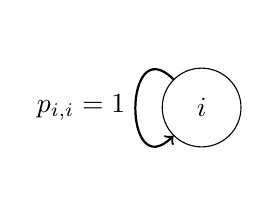
\begin{tikzpicture}
    % Définition du nœud absorbant
    \node[circle, draw, minimum size=1cm] (i) at (0,0) {$i$};
    
    % Boucle sur le nœud absorbant
    \draw[->, thick] (i) .. controls (-1,1) and (-1,-1) .. (i) node[midway, left] {$p_{i,i} = 1$};
    
\end{tikzpicture}
\end{center}

Une classe $\mathcal{C}_1$ telle que $\forall i \in \mathcal{C}_1, \forall j \notin \mathcal{C}_1, \; p_{i,j} = 0$ est une \emph{classe close} : sur le graphe, cela signifie qu’aucune arête ne sort de la classe.

\begin{center}
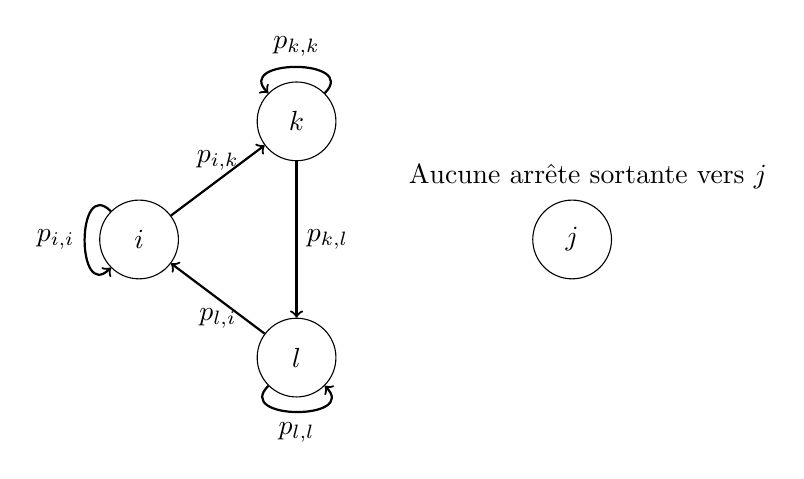
\begin{tikzpicture}
    % Définition des nœuds
    \node[circle, draw, minimum size=1cm] (i) at (0,0) {$i$};
    \node[circle, draw, minimum size=1cm] (k) at (2,1.5) {$k$};
    \node[circle, draw, minimum size=1cm] (l) at (2,-1.5) {$l$};
    \node[circle, draw, minimum size=1cm] (j) at (5.5,0) {$j$};

    % Arêtes internes à la classe C1
    \draw[->, thick] (i) -- (k) node[midway, above] {$p_{i,k}$};
    \draw[->, thick] (k) -- (l) node[midway, right] {$p_{k,l}$};
    \draw[->, thick] (l) -- (i) node[midway, below] {$p_{l,i}$};

    % Boucles sur les nœuds de la classe C1
    \draw[->, thick] (i) .. controls (-0.8,0.8) and (-0.8,-0.8) .. (i) node[midway, left] {$p_{i,i}$};
    \draw[->, thick] (k) .. controls (2.8,2.3) and (1.2,2.3) .. (k) node[midway, above] {$p_{k,k}$};
    \draw[->, thick] (l) .. controls (1.2,-2.3) and (2.8,-2.3) .. (l) node[midway, below] {$p_{l,l}$};

    % Absence d'arêtes sortantes vers j
    % État extérieur sans connexion depuis la classe close
    % Optionnel : ajout d'un message
    \node at (5.7,0.8) {Aucune arrête sortante vers $j$};

\end{tikzpicture}
\end{center}

\begin{tcolorbox}[colback=blue!5!white,colframe=blue!75!black,title=Définition]
S’il n’y a qu’une seule classe pour la relation de communication, autrement dit, si
tous les états communiquent entre eux, la chaîne est dite \emph{irréductible}.
\end{tcolorbox}

\subsubsection{Périodicité d'une chaîne markovienne}

Il s’agit d’étudier dans quelles conditions le temps qui sépare deux retours au même état $j$ est ou n’est pas multiple d’un temps minimum. C'est à cette fin que la notion de période est introduite.

\begin{tcolorbox}[colback=blue!5!white,colframe=blue!75!black,title=Définition]
Soit $j \in E$. Il est appelé \emph{période de $j$}, et on note $d(j)$, le P.G.C.D. de tous les entiers $n \geq 1$ pour lesquels $p^{(n)}_{j,j} > 0$ (par convention, $\operatorname{pgcd}(\emptyset) = +\infty$) :

\begin{equation}
 d(j) = \operatorname{pgcd}(n \geq 1, p^{(n)}_{j,j} > 0)   
\end{equation}

Si $d(j) = d \geq 2$, il est dit que $j$ est \emph{périodique de période $d$}. Si $d(j) = 1$, il est affirmé que $j$ est \emph{apériodique}. Une \emph{chaîne apériodique} est une chaîne dont tous les états sont apériodiques.
\end{tcolorbox}

Si $i \gets j$, alors il existe deux entiers $n$ et $m$ tels que $p^{(n)}_{i,j} > 0$ et $p^{(m)}_{j,i} > 0$. 
Étant donné que $i$ est de période $d(i) = d$, un entier $s \geq 1$ (multiple de $d \geq 1$) satisfait $p^{(s)}_{i,i} > 0$. 
Ainsi, 
\[
p^{(m+s+n)}_{j,j} \geq p^{(m)}_{j,i} p^{(s)}_{i,i} p^{(n)}_{i,j} > 0.
\]
La condition $p^{(s)}_{i,i} > 0$ implique $p^{(2s)}_{i,i} > 0$, ce qui entraîne également $p^{(m+2s+n)}_{j,j} > 0$. La période de $j$ divise donc $m+s+n$ et $m+2s+n$, et également leur différence $s$. En particulier, la période de $j$ divise la période $d(i)$ de $i$. De manière similaire, il est démontré que $d(i)$ divise $d(j)$, ce qui montre que $d(i) = d(j)$.


\subsubsection{Transcience et récurrence d'une chaîne markovienne}

Pour tout état $j$, qu'il soit déginé par $T_j$ le temps d’atteinte de l’état $j$ à partir de l’instant 1 ; autrement dit

\begin{equation}
T_j = \inf \{ n \geq 1 \mid X_n = j \}  
\end{equation}

Ce temps d'atteinte est un temps d'arrêt de la chaîne. Il est noté également 

\begin{equation}
N_j = \sum_{n \geq 0} \mathbbm{1}_{X_n = j} 
\end{equation}

le nombre de passages en $j$ (en comptant le point de départ). En particulier, il est constaté que 

\begin{equation}
\mathbb{P}_j(T_j < \infty) = \mathbb{P}_j(N_j \geq 1).   
\end{equation}

\begin{tcolorbox}[colback=blue!5!white,colframe=blue!75!black,title=Définition]
Il est dit que l'état $j$ est \emph{récurrent} si, partant de l’état $j$, la probabilité que la chaîne de Markov retourne à l’état $j$ en un temps fini est égale à 1, c’est-à-dire si 

\begin{equation}
\mathbb{P}_j(T_j < +\infty) = \mathbb{P}(T_j < +\infty \mid X_0 = j) = 1    
\end{equation}

Sinon, lorsque $\mathbb{P}(T_j < +\infty \mid X_0 = j) < 1$, l'état $j$ est \emph{transient} ou \emph{transitoire}.
\end{tcolorbox}


Si $j$ est récurrent, le nombre de passages en $j$ en partant de $j$ est presque sûrement
infini : $\mathbb{P}_j(N_j = +\infty) = 1$, et a fortiori $\mathbb{E}_j[N_j] = \infty$. Si $j$ est transient, le nombre de passages en $j$ en partant de $j$ (c’est-à-dire $N_j$ conditionné par $X_0 = j$)
suit une loi géométrique et est donc presque sûrement fini, et d’espérance finie. De plus, si $j$ est transient, le nombre de passages en $j$ en partant de $i$ est également presque sûrement fini et
d’espérance finie.\\

Intuitivement, si un retour presque sûr se produit au moins une fois, l'argument peut être répété après chaque retour, impliquant ainsi un retour au moins deux fois, et ainsi de suite. Cela inspire une démonstration basée sur la propriété forte de Markov, en intégrant la notion de temps
$T_j$ de premier retour en $j$.\\

Soit $k > 1$. Alors, puisque $(N_j = k) \subset (T_j < \infty)$, il est établi que, si $\mathbb{P}(T_j < \infty) \neq 0$,

\begin{equation}
    \mathbb{P}_j(N_j = k) = \mathbb{P}_j(N_j = k \mid T_j < \infty) \mathbb{P}_j(T_j < \infty).  
\end{equation}

Or,

\begin{equation}
    \begin{split}
&\mathbb{P}_j(N_j = k \mid T_j < \infty) \\
= &\mathbb{P}_j \left( \sum_{n=0}^{T_j - 1} \mathbbm{1}_{X_n = j} + \sum_{n=T_j}^{\infty} \mathbbm{1}_{X_n = j} = k \mid T_j < \infty \right) \\
= & \mathbb{P}_j \left( 1 + \sum_{n=0}^{\infty} \mathbbm{1}_{X_{T_j + n} = j} = k \mid T_j < \infty \right)
    \end{split}
\end{equation}

Il est possible alors d'appliquer la propriété de Markov forte : conditionnellement à $T_j < \infty$, la chaîne $(X_{T_j + n})$ a même loi que la chaîne partant de $j$. Ainsi,

\begin{equation}
\mathbb{P}_j(N_j = k \mid T_j < \infty) = \mathbb{P}_j \left( \sum_{n=0}^{\infty} \mathbbm{1}_{X_n = j} = k - 1 \right) = \mathbb{P}_j(N_j = k - 1)  
\end{equation}

Finalement, pour tout $k > 1$, 

\begin{equation}
\mathbb{P}_j(N_j = k) = \mathbb{P}_j(N_j = k - 1) \mathbb{P}_j(T_j < \infty)   
\end{equation}

La suite $(P_j(N_j = k))_{k \geq 1}$ est donc géométrique.

Si $j$ est récurrent : alors $\mathbb{P}_j(T_j < \infty) = 1$, donc cette suite est constante. Or $\sum_{k \geq 1} \mathbb{P}_j(N_j = k) = \mathbb{P}_j(N_j < \infty)$. Il en résulte une série de termes constants convergente : chaque terme est donc nul, et 
finalement, il est établi que $\mathbb{P}_j(N_j = +\infty) = 1$.\\

Si $j$ est transitoire : alors $q := \mathbb{P}_j(T_j < \infty) < 1$. Il est déduit pour tout $k$

\begin{equation}
\mathbb{P}_j(N_j = k) = \mathbb{P}_j(N_j = 1) q^{k - 1}
\end{equation}

Il est possible de vérifier facilement $\mathbb{P}_j(N_j = 1) = \mathbb{P}_j(T_j = \infty) = 1 - q$. Par conséquent, conditionnellement à $X_0 = j$, $N_j$ suit bien une loi géométrique de paramètre $\mathbb{P}_j(T_j = \infty)$, et est bien d’espérance finie.

Enfin, toujours si $j$ est transitoire : si $j$ n’est pas accessible à partir de $i \in E$, alors le nombre de passages
en $j$ en partant de $i$ est presque sûrement nul. Si $i \rightarrow j$ et $i \neq j$, en notant toujours $T_j$ le temps d’atteinte de $j$, on a grâce à la propriété de Markov forte pour tout $k \geq 1$ :

\begin{equation}
\mathbb{P}_i(N_j \geq k) = \mathbb{P}_i(N_j \geq k \mid T_j < \infty) \mathbb{P}_i(T_j < \infty) = \mathbb{P}_i \left( \sum_{n \geq T_j} \mathbbm{1}_{X_n = j} \geq k \mid T_j < \infty \right) \mathbb{P}_i(T_j < \infty)
\end{equation}

Ainsi,

\begin{equation}
\mathbb{P}_j(N_j \geq k) \mathbb{P}_i(T_{ij} < \infty) \leq \mathbb{P}_j(N_j \geq k).    
\end{equation}

\begin{tcolorbox}[colback=yellow!5!white,colframe=yellow!75!black, title=Corollaire]
$j$ est récurrent si et seulement si $\displaystyle{\sum_{n \geq 0}} p^{(n)}_{j,j}$ diverge.

$j$ est transitoire si et seulement si $\displaystyle{\sum_{n \geq 0}} p^{(n)}_{j,j}$ converge.

De plus, si $j$ est transitoire, alors $p^{(n)}_{i,j} \to 0$ quel que soit $i$.
\end{tcolorbox}

Il suffit, en vertu de la proposition précédente, de vérifier que :
\[
\mathbb{E}_j[N_j] = \sum_{n \geq 0} p^{(n)}_{j,j}.
\]
Or, 
\[
\mathbb{E}_j[N_j] = \mathbb{E}\left[\sum_{n \geq 0} \mathbf{1}_{X_n = j} \mid X_0 = j\right].
\]
L'espérance et la série peuvent être permutées (car il s'agit d'une série à termes positifs), ce qui donne
\[
\mathbb{E}_j[N_j] = \sum_{n \geq 0} \mathbb{E}\left[\mathbf{1}_{X_n = j} \mid X_0 = j\right] = \sum_{n \geq 0} \mathbb{P}(X_n = j \mid X_0 = j).
\]
Par définition, $\mathbb{P}(X_n = j \mid X_0 = j) = p^{(n)}_{j,j}$. Ainsi, 
\[
\mathbb{E}_j[N_j] = \sum_{n \geq 0} p^{(n)}_{j,j}.
\]

Enfin, si $j$ est transitoire, le nombre de passages en $j$ en partant de $i$ est d'espérance finie. Par conséquent, il est obtenu de manière similaire que 
\[
\mathbb{E}_i[N_j] = \sum_{n \geq 0} \mathbb{E}\left[\mathbf{1}_{X_n = j} \mid X_0 = i\right] = \sum_{n \geq 0} p^{(n)}_{i,j}.
\]
Cette série converge, ce qui implique que son terme général tend vers $0$.


\begin{tcolorbox}[colback=green!5!white,colframe=green!75!black,title=Proposition]
    \textbf{Décomposition de l’espace d’états.}\\

    L’espace d’états se partitionne en classe d’équivalence pour la relation de communication.
    
    \begin{itemize}
        \item Une classe non close est transiente.
        \item Une classe close finie est récurrente.
    \end{itemize}
    
    En particulier, pour les chaînes de Markov à espace d’états finis :
    \begin{itemize}
        \item Les classes récurrentes sont les classes closes.
        \item Les classes transientes sont les classes non closes.
    \end{itemize}
    
    Il est déduit également qu’une chaîne de Markov à espace d’états fini admet au moins un état récurrent.
\end{tcolorbox}    

Soit $C$ une classe non close : il existe donc $i \in C$ et $j \notin C$ tels que $p_{ij} \neq 0$. 
Cependant, $i$ et $j$ ne communiquent pas : puisque $i \nleftrightarrow j$, $i$ n’est pas accessible à partir de $j$. 
Par conséquent, pour tout $n$, 
\[
\mathbb{P}(X_n = i \mid X_1 = j) = 0.
\]
Il en résulte que 
\[
\mathbb{P}(T_i < \infty \mid X_1 = j) = 0.
\]
Finalement, 
\[
\mathbb{P}(T_i = +\infty \mid X_0 = i) \geq \mathbb{P}(T_i = +\infty \mid X_0 = i, X_1 = j) \mathbb{P}(X_1 = j \mid X_0 = i) = p_{ij} > 0.
\]
Il s'ensuit que $i$ est transitoire et que $C$ est transitoire.\\

Considérons maintenant une classe $C$ close et finie. Une démonstration par l'absurde est utilisée pour montrer que tous les états de $C$ ne peuvent pas être transitoires. Supposons que tous les états de $C$ soient transitoires. Soit $i \in C$. Étant donné que la chaîne reste dans $C$ en partant de $i$, il est vérifié que :
\[
\mathbb{P}_i\left(\sum_{j \in C} N_j = \infty\right) = 1.
\]
Cette somme étant finie, il en découle que 
\[
\mathbb{P}_i\left(\exists j \in C, N_j = \infty\right) = 1.
\]
Cependant, pour tout $j \in C$, il a été supposé que $j$ est transitoire, ce qui implique que 
\[
\mathbb{P}_i(N_j = \infty) = 0.
\]
Une contradiction est obtenue.\\

Ainsi, toute classe close d'une chaîne à espace d’états fini est récurrente. Une chaîne à espace d’états fini possède au moins une classe close et donc au moins un état récurrent. En particulier, une chaîne de Markov à espace d’états fini n’ayant qu’une seule classe est automatiquement récurrente.

\subsubsection{Lois de probabilités stationnaires}

Dans ce paragraphe, les lois de probabilité $\mu$ sur l’ensemble des états $E$ sont notées comme des vecteurs lignes 
\[
\mu = (\mu_0, \mu_1, \mu_2, \dots),
\]
où $0 \leq \mu_i \leq 1$ et $\sum_i \mu_i = 1$.

\begin{tcolorbox}[colback=blue!5!white,colframe=blue!75!black,title=Définition]
    Soit $\nu$ une loi de probabilité sur l’ensemble des états. Elle est dite \textit{stationnaire}, ou \textit{invariante}, si $\nu = \nu P$ ou, de façon équivalente, si pour tout $j \in E$ on a
    \begin{equation}
        \nu_j = \sum_{i \in E} \nu_i p_{i,j}
    \end{equation}
    Si $\nu$ est une loi de probabilité stationnaire et si $i$ est un état transitoire, alors $\nu(i) = 0$. En particulier, si un processus n’a que des états transitoires, alors il n’admet pas de loi de probabilité stationnaire.
    \end{tcolorbox}

$\mu$ peut également être caractérisé comme un vecteur propre de $P^\top$ associé à la valeur propre $1$. Supposons qu'une loi de probabilité stationnaire $\nu$ existe ; pour tout $n \geq 0$, il est vérifié que 
\[
\nu = \nu P^{(n)}.
\]
Il en résulte que, si $\nu$ est utilisée comme loi de probabilité initiale, c’est-à-dire si $\mu^{(0)}_i = \mathbb{P}(X_0 = i) = \nu_i$, alors la loi de probabilité de $X_n$, donnée par 
\[
\mu^{(n)} = \mu^{(0)} P^{(n)},
\]
est indépendante de $n$ et est égale à $\mu^{(0)}$. Ainsi, il est vérifié que 
\[
\mathbb{P}(X_n = i) = \mathbb{P}(X_0 = i) = \nu_i.
\]

De manière générale, lorsque $\nu$ est utilisée comme loi de probabilité initiale, la chaîne de Markov est transformée en un processus stationnaire. Cela signifie que, pour tout $n \geq 0$ et tout $k \geq 0$, il est satisfait que 
\[
\mathcal{L}(X_n, \dots, X_{n+k}) = \mathcal{L}(X_0, \dots, X_k).
\]

D'autre part, si $X_n$ converge en loi vers une loi $\nu$, il en découle que 
\[
\nu_0 P^n \to \nu.
\]
En considérant la suite $(\nu_0 P^n)P$, il est montré que $\nu = \nu P$, et $\nu$ est ainsi une loi invariante. Par conséquent, une forte liaison existe entre les lois stationnaires et le comportement asymptotique de la chaîne.\\

Dans le cas dénombrable, il n’est pas garanti qu'une probabilité stationnaire existe. Dans certains cas, une infinité de probabilités stationnaires peuvent exister.

\begin{tcolorbox}[colback=green!5!white,colframe=green!75!black,title=Proposition]
Si $\nu$ est une loi de probabilité stationnaire et si $i$ est un état transitoire, il est vérifié que $\nu(i) = 0$. 

En particulier, si un processus ne contient que des états transitoires, aucune loi de probabilité stationnaire ne peut être admise.
\end{tcolorbox}    

Soit $\nu$ une loi de probabilité stationnaire et $i$ un état transitoire. Il est vérifié que, pour tout $n$, $\nu P^n = \nu$, ce qui donne 
\[
\nu_i = \sum_j \nu_j p^{(n)}_{ji}.
\]

Étant donné que $i$ est transitoire, $p^{(n)}_{ji}$ tend vers $0$. La série et la limite peuvent être inversées par le théorème de convergence dominée, car $|p^{(n)}_{ji}| \leq 1$ et $\sum_j \nu_j = 1$. Par conséquent, il est obtenu que $\nu_i = 0$.\\

Ainsi, si un processus ne contient que des états transitoires, une loi de probabilité stationnaire satisferait $\nu_i = 0$ pour tout $i \in E$, ce qui est impossible.

\paragraph{Lois invariantes.}

Soit $(X_n)$ une chaîne de Markov à ensemble d’états fini. Alors elle possède au moins une loi de probabilité stationnaire :

\begin{itemize}
\item De plus, si $(X_n)$ est irréductible, alors la loi de probabilité stationnaire est unique. Elle est 
noté  $\nu$; elle vérifie, pour tout $i$ dans $E$, que
    
\begin{equation}
    \nu(i) = \frac{1}{\mathbb{E}_i [T_i]} > 0 
\end{equation}
    
où $T_i$ est le temps de premier retour en $i$.

\item Si de plus $(X_n)$ est irréductible et apériodique, alors $P^n$ converge vers la matrice dont
toutes les lignes sont constantes égales à $\nu$. En particulier, quelle que soit la loi de $X_0$, $X_n$
converge en loi vers $\nu$.
\end{itemize}

\begin{tcolorbox}[colback=blue!5!white,colframe=blue!75!black,title=Définition]
Soit une chaîne de Markov irréductible d’espace d’états fini. Il est noté $\mu$ son unique loi de probabilité invariante. Il est vérifié que, pour toute fonction $f$ sur $E$,
\[
\lim_{n \to \infty} \frac{1}{n} \sum_{k=0}^{n-1} f(X_k) = \frac{\displaystyle{\sum_{i \in E}} f(i) \mu(i)}{\mathbb{E}_i[T_i]} = \int f \, d\mu \quad \text{p.s.}
\]

De plus,
\[
\sqrt{n} \left( \frac{f(X_0) + \cdots + f(X_{n-1})}{n} - \int f \, d\mu \right)
\]
converge en loi vers une loi normale centrée.
\end{tcolorbox}

\paragraph{États récurrents nuls et positifs.} Le cas dénombrable nécessite une classification des états encore plus fine, ce qui conduit à la définition de la notion de positivité. Il a été rappelé qu’un état $j$ est dit récurrent si :
\[
\mathbb{P}(T_j < +\infty \mid X_0 = j) = 1.
\]
L’étude se porte maintenant sur l’espérance de ce temps de retour.

\begin{tcolorbox}[colback=blue!5!white,colframe=blue!75!black,title=Définition]
Pour $j$, un état d’une chaîne de Markov, le temps d’atteinte moyen dans $j$ à partir de $i$ est défini par :
\[
M_{i,j} = \mathbb{E}(T_j \mid X_0 = i) = \sum_{n \geq 1} n \mathbb{P}(T_j = n \mid X_0 = i) = \sum_{n \geq 1} n f^{(n)}_{i,j}.
\]

Pour $j$, un état d’une chaîne de Markov, la quantité $M_{j,j}$ est appelée \textit{temps de retour moyen} dans $j$, et $\frac{1}{M_{j,j}}$ représente la \textit{fréquence moyenne de retour} en $j$.\\

Un état $j$ est dit \textit{positif} si $M_{j,j} < +\infty$ ; sinon, $j$ est dit \textit{nul}.
\end{tcolorbox}

Si $j$ est transitoire, il est établi que $\mathbb{P}(T_j = +\infty \mid X_0 = j) > 0$, ce qui implique $M_{j,j} = +\infty$. Ainsi, un état transitoire est nécessairement \textit{nul}.\\

Les états récurrents nuls se situent entre les états transitoires et les états récurrents positifs. Ces états sont récurrents, mais leur temps moyen de récurrence est infini, comme pour les états transitoires.\\

Un critère permettant de caractériser la positivité d’un état récurrent sera présenté avec une démonstration partielle ultérieurement.\\

Un état récurrent $j$ d’une chaîne de Markov est \textit{nul} si et seulement si :
\[
\lim_{n \to \infty} p^{(n)}_{j,j} = 0.
\]

La positivité, comme la nullité, est une propriété de classe.\\

En effet, soit $i$ un état récurrent nul et $j$ un autre état appartenant à la même classe que $i$. Puisque $i$ et $j$ communiquent, il existe des entiers $n_0$ et $n_1$ tels que :
\[
p^{(n_0)}_{i,j} > 0 \quad \text{et} \quad p^{(n_1)}_{j,i} > 0.
\]
Il en résulte que :
\[
p^{(n_0 + m + n_1)}_{i,i} \geq p^{(n_0)}_{i,j} \cdot p^{(m)}_{j,j} \cdot p^{(n_1)}_{j,i}.
\]
En faisant tendre $m$ vers l’infini, la nullité de $i$ entraîne celle de $j$.\\

Ainsi, une classe d’équivalence d’une chaîne de Markov est soit \textit{transiente}, soit \textit{récurrente nulle}, soit \textit{récurrente positive}.


\begin{tcolorbox}[colback=green!5!white,colframe=green!75!black,title=Proposition]
Si l’espace des états est fini, les états récurrents sont tous positifs.
\end{tcolorbox}  

Soit $i$ un état récurrent. Si $i$ est absorbant (seul dans une classe), alors pour tout $n \geq 0$, $p^{(n)}_{i,i} = 1$, et, par le théorème 35, $i$ est récurrent positif. Si $i$ n’est pas seul dans sa classe, une communication existe au moins avec un autre état $j$. Supposons que cette classe récurrente, notée $C$, soit nulle.\\

Soit $n_0$ tel que $p^{(n_0)}_{j,i} > 0$. Il est vérifié que :
\[
p^{(n_0 + m)}_{i,i} \geq p^{(m)}_{i,j} \cdot p^{(n_0)}_{j,i}.
\]
Par le théorème 35, il en résulte que $\lim_{m \to +\infty} p^{(m)}_{i,j} = 0$. Par conséquent, puisque l’espace des états est fini, la classe $C$ l’est également, et il est montré que :
\[
\lim_{m \to +\infty} \sum_{j \in C} p^{(m)}_{i,j} = 0.
\]
Cependant, comme il est impossible de quitter une classe récurrente, une contradiction apparaît avec le fait que :
\[
1 = \sum_{j \in E} p^{(m)}_{i,j} = \sum_{j \in C} p^{(m)}_{i,j}.
\]

\begin{tcolorbox}[colback=yellow!5!white,colframe=yellow!75!black, title=Corollaire]
Une chaîne de Markov irréductible sur un espace d’états fini est forcément récurrente
positive.
\end{tcolorbox}

\paragraph{Mesures stationnaires.} Soit $(X_n)$ une chaîne irréductible récurrente. Une mesure invariante sera explicitée, bien qu’elle ne constitue pas nécessairement une probabilité. Dans le cas où la chaîne est positive, il sera démontré que cette mesure est finie, ce qui implique l’existence d’une loi de probabilité stationnaire. Il sera par ailleurs établi, dans un second temps, que cette loi de probabilité stationnaire est unique.


\begin{tcolorbox}[colback=blue!5!white,colframe=blue!75!black,title=Définition]
Soit $(X_n)$ une chaîne irréductible récurrente avec un nombre au plus dénombrable d’états, et soit $i \in E$. Pour tout $j \in E$, il est défini
\[
u^i_j = \mathbb{E} \left[\sum_{n \geq 0} \mathbb{1}_{\{X_n = j, n \leq T_i - 1\}} \mid X_0 = i \right].
\]

La mesure $\nu^i$ définie par $\nu^i(j) = u^i_j$ est stationnaire. Elle vérifie les propriétés suivantes :
\[
\nu^i(i) = 1, \quad \nu^i(j) < \infty \; \text{pour tout } j, \quad \text{et} \quad \nu^i(E) = \mathbb{E}[T_i \mid X_0 = i].
\]

Il est établi que toutes les mesures stationnaires sont proportionnelles. Ainsi :
\begin{itemize}
    \item Si la chaîne est irréductible récurrente positive, $\nu^i(E) < \infty$ et il existe une unique loi de probabilité stationnaire donnée par :
    \[
    \mu(i) = \frac{1}{\mathbb{E}[T_i \mid X_0 = i]} = \frac{1}{M_{i,i}}.
    \]
    \item Si la chaîne est irréductible récurrente nulle, $\nu^i(E) = +\infty$ et aucune loi de probabilité stationnaire n’existe.
\end{itemize}
\end{tcolorbox}

$u^i_j$ est défini comme l’espérance du temps passé en $j$ entre deux passages successifs en $i$.\\

Il est d’abord établi que, la chaîne étant récurrente, $T_i < \infty$ presque sûrement. De plus, l'irréductibilité de la chaîne implique que $u^i_j > 0$ pour tout $j$. Il est également vérifié que $u^i_i = 1$.\\

La stationnarité de $\nu^i$ est maintenant démontrée. L'expression suivante est utilisée :
\[
u^i_j = \mathbb{E} \left[\sum_{n \geq 0} \mathbf{1}_{\{X_n = j, n \leq T_i - 1\}} \mid X_0 = i \right] 
= \sum_{n \geq 0} \mathbb{P}(X_n = j, n \leq T_i - 1 \mid X_0 = i).
\]

Dans le cas où $j \neq i$, il est obtenu que :
\[
u^i_j = \sum_{n \geq 1} \mathbb{P}(X_n = j, n \leq T_i - 1 \mid X_0 = i) = \sum_{n \geq 1} \mathbb{P}(X_n = j, n \leq T_i \mid X_0 = i).
\]

Pour $i = j$, il est également établi que :
\[
u^i_i = 1 + \sum_{n \geq 1} \mathbb{P}(X_n = i, n \leq T_i \mid X_0 = i).
\]

Finalement, pour tout $j$, il est obtenu que :
\[
u^i_j = \mathbb{P}(X_1 = j, 1 \leq T_i \mid X_0 = i) + \sum_{n \geq 2} \mathbb{P}(X_n = j, n \leq T_i \mid X_0 = i).
\]

Pour $n \geq 2$, il est démontré que :
\[
\mathbb{P}(X_n = j, n \leq T_i \mid X_0 = i) = \sum_{k \neq i} \mathbb{P}(X_n = j \mid X_{n-1} = k, n \leq T_i, X_0 = i) \cdot \mathbb{P}(X_{n-1} = k, n \leq T_i \mid X_0 = i).
\]

Chaque terme est décomposé en fonction des probabilités de transition conditionnelles. Cela montre que $\nu^i$ satisfait les propriétés de stationnarité.\\

L’événement $\{n \leq T_i\} = \{X_1 \neq i, \dots, X_{n-1} \neq i\}$ appartient à la tribu $\mathcal{F}_{n-1}$. Par conséquent, 
\[
\mathbb{P}(X_n = j \mid X_{n-1} = k, n \leq T_i, X_0 = i) = p_{k,j}.
\]
Il en résulte que :
\[
u^i_j = p_{i,j} + \sum_{n \geq 2} \sum_{k \neq i} p_{k,j} \mathbb{P}(X_{n-1} = k, n \leq T_i \mid X_0 = i).
\]
En réorganisant, il est obtenu :
\[
u^i_j = p_{i,j} + \sum_{k \neq i} p_{k,j} \sum_{n \geq 2} \mathbb{P}(X_{n-1} = k, n \leq T_i \mid X_0 = i).
\]
Finalement, cela devient :
\[
u^i_j = p_{i,j} + \sum_{k \neq i} p_{k,j} u^i_k = \sum_k u^i_k p_{k,j}.
\]
Ainsi, $\nu^i$ est bien une mesure invariante. 

Par conséquent, $\nu^i$ est également invariante par $P^n$ pour tout entier $n$. Puisque $j \neq i$ et que la chaîne est irréductible, il existe $m$ tel que $p^{(m)}_{j,i} > 0$. Il est donc établi que :
\[
1 = u^i_i = \sum_k u^i_k p^{(m)}_{k,i} \geq u^i_j p^{(m)}_{j,i}.
\]
Il en découle que $\nu^i(j)$ est bien fini pour tout $j$.

Par ailleurs, comme tous les termes sont positifs, il est possible d’échanger les séries et les espérances. Ainsi :
\[
\sum_j u^i_j = \mathbb{E} \left[\sum_{j} \sum_{n \geq 0} \mathbf{1}_{\{X_n = j, n \leq T_i - 1\}} \mid X_0 = i \right] = \mathbb{E}[T_i \mid X_0 = i] = M_{i,i}.
\]
Si $i$ est récurrent positif, alors $M_{i,i} < \infty$ et $\mu = \frac{\nu^i}{M_{i,i}}$ est bien une loi de probabilité stationnaire.\\

Il reste à démontrer que les mesures invariantes sont uniques à coefficient multiplicatif près. Soit $\mu$ une mesure invariante non nulle. Il est d'abord montré que $\mu$ charge tous les états. En effet, il existe un état $i$ tel que $\mu(i) > 0$. Pour tout état $k$, il existe $m$ tel que $p^{(m)}_{i,k} > 0$. Par conséquent :
\[
\mu(k) = \sum_l \mu(l) p^{(m)}_{l,k} \geq \mu(i) p^{(m)}_{i,k} > 0.
\]
Il suffit alors de vérifier que $\frac{\mu}{\mu(i)}$, qui satisfait $\mu(i) = 1$, est égale à $\nu^i$, et est donc bien déterminée. On écrit :
\[
\mu(j) = p_{j,i} + \sum_{k \neq i} \mu(k) p_{j,k}.
\]
Il est obtenu que, pour tout $j$, $\mu(j) \geq p_{j,i}$. En reportant dans la somme précédente, il est démontré que :
\[
\mu(j) \geq p_{j,i} + \sum_{k \neq i} p_{k,i} p_{j,k} \geq p_{j,i} + \mathbb{P}(X_2 = j, T_i \geq 2 \mid X_0 = i).
\]
Par récurrence, il est finalement montré que, pour tout $n$ :
\[
\mu(j) \geq \mathbb{P}(X_1 = j, T_i \geq 1) + \mathbb{P}(X_2 = j, T_i \geq 2) + \dots + \mathbb{P}(X_n = j, T_i \geq n).
\]
En faisant tendre $n$ vers l’infini, il est conclu que $\mu \geq \nu^i$.\\

Supposons que $\mu \neq \nu^i$, c’est-à-dire qu’il existe $j$ tel que $\mu(j) < \nu^i_j$. Alors, $\mu - \nu^i$ est une mesure invariante non nulle, et il est vérifié que $\mu(i) - \nu^i(i) = 0$. Cela est impossible, car une mesure invariante pour une chaîne irréductible charge tous les points.\\

Ainsi, si la chaîne est irréductible récurrente positive, la loi de probabilité invariante est unique et peut être obtenue en normalisant $\nu^i$ par $\nu^i(E)$. Cette loi ne dépend pas du choix de $i$ et vérifie, pour tout $i$ :
\[
\mu(i) = \frac{\nu^i(i)}{\nu^i(E)} = \frac{1}{\nu^i(E)} = \frac{1}{M_{i,i}}.
\]

\paragraph{Définition des variables aléatoires :}
\begin{itemize}
    \item $N_n(j) = \displaystyle{\sum_{k=0}^{n-1} \mathbf{1}\{X_k = j\}}$ : \
    C'est le nombre de fois que le processus séjourne dans l'état $j$ dans l'intervalle de temps $[0, n-1]$.
    \item $F_n(j) = \displaystyle{\frac{1}{n} \sum_{k=0}^{n-1} \mathbf{1}\{X_k = j\} = \frac{N_n(j)}{n}}$ : \
    C'est la fréquence de séjour dans l'état $j$ dans l'intervalle de temps $[0, n-1]$.
\end{itemize}

Si les $X_n$ étaient indépendantes et de même loi, il pourrait être appliqué la loi forte des grands nombres à la suite $F_n$. Cependant, pour les chaînes de Markov, la loi commune des $(X_n)$ dans la LFGN est remplacée par la loi invariante des $X_n$.\\

\begin{tcolorbox}[colback=blue!5!white,colframe=blue!75!black,title=Définition]
Si une chaîne de Markov est irréductible et de loi initiale quelconque, alors pour tout état $j$, on a :
\[
F_n(j) = \frac{N_n(j)}{n} \longrightarrow \frac{1}{\mathbb{E}[T_j|X_0 = j]} \quad \text{p.s.}
\]
\end{tcolorbox}

Pour simplifier les notations, les dépendances en $j$ sont oubliées.\\

Si $j$ est un état transitoire, la suite $(N_n)$ est presque sûrement bornée, donc $\frac{N_n}{n}$ tend vers $0$. De plus, il est vérifié que $\mathbb{E}[T_j | X_0 = j] = \infty$, ce qui valide la première égalité.\\

Si $j$ est récurrent, la suite $(N_n)$ est croissante et tend vers l’infini. Le temps d’atteinte de $j$ est presque sûrement fini quel que soit le point de départ, et il peut donc être supposé que le processus démarre en $j$. La suite $T^{(n)}$ des passages successifs en $j$ est alors considérée (avec $T^{(1)} = T_j$, le temps du premier retour en $j$). Par définition, il est obtenu :
\[
T^{(N_n-1)} \leq n \leq T^{(N_n)}.
\]
Par conséquent :
\[
\frac{T^{(N_n-1)}}{n} \leq \frac{N_n}{n} \leq \frac{T^{(N_n)}}{N_n}.
\]

La propriété de Markov forte implique que les incréments $T^{(k)} - T^{(k-1)}$ (pour $k$ allant de $1$ à $n$, avec $T^{(0)} = 0$) sont indépendants et identiquement distribués selon la loi de $T^{(1)} = T_j$. Si $j$ est un état positif, la loi forte des grands nombres peut être appliquée : 
\[
\frac{T^{(n)}}{n} \xrightarrow{p.s.} \mathbb{E}[T_j | X_0 = j] = M_{j,j}.
\]
Si $j$ est un état nul, l’espérance précédente est infinie, mais la propriété reste valide par convergence monotone.\\

Étant donné que $N_n$ converge presque sûrement vers l’infini, il est finalement obtenu que :
\[
\frac{T^{(N_n)}}{N_n} \xrightarrow{p.s.} M_{j,j}.
\]

Puisque $\frac{N_n - 1}{N_n} \xrightarrow{p.s.} 1$, il est également obtenu que :
\[
\frac{T^{(N_n-1)}}{N_n} \xrightarrow{p.s.} M_{j,j}.
\]

En conclusion, 
\[
F_n(j) = \frac{N_n}{n} \xrightarrow{p.s.} \frac{1}{\mathbb{E}_j[T_j]}.
\]

Après avoir posé les bases théoriques des chaînes de Markov, notamment leur structure, leurs propriétés de convergence et leur théorème ergodique, il est maintenant nécessaire d’explorer leurs applications dans le cadre des modèles économétriques à changement de régime markovien. Plus particulièrement, dans le cas multivarié du modèle Vector AutoRegressive (MS-VAR) qui capture les changements de régimes dans les séries temporelles multivariées. Ces modèles exploitent les propriétés des chaînes de Markov pour modéliser les changement de régimes, tout en prenant en compte l’existence de leur latence.

\subsection{Modèle Markov Switching-VAR}

Les modèles de Markov-Switching Vector Autoregressive (MS-VAR) ont été développés pour modéliser les dynamiques économiques et financières, notamment dans des contextes où les régimes changent de manière imprévisible. Ces modèles permettent aux paramètres de varier selon un processus de chaîne de Markov, capturant ainsi de manière flexible les changements structurels dans les séries temporelles. Le modèle MS-VAR a été initialement popularisé par \cite[1989]{Hamilton}, qui a démontré comment les changements de régime peuvent être intégrés pour refléter des dynamiques non linéaires et des structures économiques changeantes. \cite[1994]{Hamilton} a ensuite étendu cette approche dans un cadre VAR avec des innovations structurelles, où les régimes influencent les paramètres autorégressifs et la variance des chocs. Ces régimes représentent souvent des phases économiques distinctes, comme des périodes de récession ou de croissance, rendant le modèle particulièrement adapté à l'analyse macroéconomique.\\

La suite de cette section détaille les fondements théoriques et les extensions des modèles MS-VAR. Elle commence par la spécification du modèle et l'introduction des régimes latents, qui capturent les changements structurels sous-jacents dans les séries temporelles. Ensuite, une typologie complète des variantes du modèle MS-VAR est présentée, incluant des versions spécifiques comme MSIAH(m)-VAR(l) ou MSIAH(m)-VARX(p, q), qui ajoutent des fonctionnalités comme des variables exogènes ou des interactions complexes entre les paramètres et les régimes.\\

L'analyse se poursuit avec une exploration des vecteurs d'innovations et des matrices de variance-covariance, en mettant l'accent sur des outils comme la décomposition de Cholesky pour comprendre la structure des chocs et leurs interactions. Enfin, l'étude des moments conditionnels et des réponses aux chocs complète cette section. Des outils analytiques comme les Generalized Impulse Response Functions (GIRF) de premier et de second ordre, ainsi que la décomposition de la variance conditionnelle et le spillover, sont introduits pour illustrer la manière dont les modèles MS-VAR capturent les dynamiques complexes des chocs structurels.
\\

Il est à noter que d'autres travaux, tels que ceux de \cite[1997]{Krolzig}, ont perfectionné les modèles MS-VAR en introduisant la notation MSIAH(m)-VAR(l), où chaque composante du modèle peut varier selon le régime, qu'il s'agisse des intercepts, des coefficients autorégressifs, ou des variances conditionnelles. \cite[2015]{Bianchi} et \cite[2013]{Bianchi et Civelli} ont également contribué à cette littérature en explorant les moments et les réponses impulsionnelles conditionnelles, fournissant ainsi une base analytique pour des analyses plus approfondies des chocs structurels et de la dynamique de volatilité dans les modèles MS-VAR .
\\

Enfn, les applications de ces modèles vont au-delà de la macroéconomie traditionnelle. Par exemple, \cite[2014]{Hubrich et Tetlow} ont utilisé des modèles MS-VAR pour étudier l'impact des crises financières sur les variables macroéconomiques, en intégrant des régimes de stress financiers et leurs effets sur la transmission des chocs . \cite[2012]{Ang et Timmermann} ont quant à eux exploré une forme spécifique de modèles à changement de régime appliquée aux séries temporelles univariées, démontrant que la moyenne du régime spécifique peut être intégrée pour mieux capturer les caractéristiques non linéaires des données économiques.\\

Ce paragraphe s'appuie sur les travaux récents de \cite[2023]{Kole et Van Dijk} mais aussi sur le papier de \cite[2013]{Binder et Gross}. 

\subsubsection{Spécification du modèle}

Le modèle Markov-Switching Vector Autorégressif (MS-VAR) avec $m$ régimes d'ordre 1 peut être spécifié comme :

\begin{equation}
    \bm{y_t} = \bm{c}_{S_t} + \bm{\Phi}_{S_t} \bm{y}_{t-1} + \bm{\Lambda}_{S_t} \bm{\epsilon_t},
\end{equation}

où :
\begin{itemize}
    \item $\bm{y_t}$ est le vecteur de variables dépendantes de dimension $n \times 1$,
    \item $S_t$ est un processus de chaîne de Markov de premier ordre avec $m$ états distincts,
    \item $\bm{c}_{S_t}$ est le vecteur intercept spécifique au régime de dimension $n \times 1$, $ \bm{c}_{S_t} = \begin{pmatrix} 
c_{1, S_t} \\
c_{2, S_t} \\
\vdots \\
c_{n, S_t} 
\end{pmatrix}$
    \item $\bm{\Phi}_{S_t}$ est la matrice des coefficients autorégressifs spécifiques au régime de dimension $n \times n$, $\bm{\Phi}_{S_t} = 
    \begin{pmatrix}
        \phi_{S_t,11} & \cdots & \phi_{S_t,1n} \\
        \vdots & \ddots & \vdots \\
        \phi_{S_t,n1} & \cdots & \phi_{S_t,nn}
    \end{pmatrix}$
    \item $\bm{\Lambda}_{S_t}$ est la matrice de volatilité spécifique au régime de dimension $n \times n$,\\ $\bm{\Lambda}_{S_t} = 
    \begin{pmatrix}
        \lambda_{S_t,11} & \cdots & \lambda_{S_t,1n} \\
        \vdots & \ddots & \vdots \\
        \lambda_{S_t,n1} & \cdots & \lambda_{S_t,nn}
    \end{pmatrix}$
    \item $\bm{\epsilon_t} \sim N(0, \bm{I_n})$ est un vecteur de termes d'erreur \textit{(chocs idiosyncratiques)} de dimension $n \times 1$.
\end{itemize}

\subsubsection{Régimes latents}

Le processus de Markov latent \( S_t \) détermine le régime en cours et prend des valeurs parmi \(\{1, 2, \dots, m\}\), où \( m \) est le nombre de régimes possibles. Ce processus de premier ordre est gouverné par une matrice de transition \( \mathcal{P} \), définie par :

\begin{equation}
    \mathcal{P} = 
    \begin{pmatrix}
        p_{11} & p_{12} & \cdots & p_{1m} \\
        p_{21} & p_{22} & \cdots & p_{2m} \\
        \vdots & \vdots & \ddots & \vdots \\
        p_{m1} & p_{m2} & \cdots & p_{mm}
    \end{pmatrix},
\end{equation}

où chaque élément \( p_{ij} \) représente la probabilité de transition du régime \( j \) au régime \( i \), soit :

\[
p_{ij} = \mathbb{P}(S_t = i \mid S_{t-1} = j), \quad \text{avec } \sum_{i=1}^m p_{ij} = 1.
\]

Le processus de Markov est irréductible et ergodique, ce qui signifie que le modèle peut potentiellement atteindre n'importe quel régime à partir de n'importe quel autre régime sur une période infinie. Ce processus est régi par une première chaîne de Markov d'ordre 1, ce qui implique que :

\[
\mathbb{P}(S_t = i \mid S_{t-1}, S_{t-2}, \dots, S_0) = \mathbb{P}(S_t = i \mid S_{t-1}).
\]

La matrice de transition \( P \) est centrale pour décrire la dynamique des régimes. Chaque ligne de la matrice correspond à un régime précédent \( S_{t-1} \), tandis que chaque colonne représente un régime actuel \( S_t \). Par exemple, si \( P \) est une matrice \( 2 \times 2 \), les éléments sont :

\[
\mathcal{P} = \begin{pmatrix} 
p_{11} & p_{12} \\
p_{21} & p_{22} 
\end{pmatrix}
\]

Dans ce cas :
\begin{itemize}
    \item \( p_{11} \) est la probabilité que le modèle reste dans le régime 1 si le régime précédent était également le régime 1.
    \item \( p_{12} \) est la probabilité que le modèle passe du régime 1 au régime 2.
    \item \( p_{21} \) et \( p_{22} \) ont des interprétations similaires pour le passage et le maintien dans le régime 2.
\end{itemize}

L'état de long terme ou la distribution stationnaire des régimes \( \pi \) peut être déterminé en résolvant \( \pi \mathcal{P} = \pi \) avec la condition de normalisation \( \sum_{i=1}^m \pi_i = 1 \). Cela donne une idée des fréquences d'apparition des régimes à long terme, indépendamment des conditions initiales.

\subsubsection{Typologie des modèles MS-VAR}

Le modèle précédement spécifié peut être assimilé à un MSIAH(m)-VAR(1) car les erreurs, intercepts et coefficients autorégressifs varient entre les régimes. Également, il est possible de généraliser la spécification pour $p$ retards : 

\begin{equation}
    \bm{y_t} = \bm{c}_{S_t} + \sum_{i=1}^{p} \bm{\Phi}_{S_t, i} \bm{y_{t-i}} + \bm{\varepsilon_t},
\end{equation}

\paragraph{MS(m)-VAR(p)}

\begin{equation}
    \bm{y_t} = \bm{c} + \sum_{i=1}^{p} \bm{\Phi}_{S_t, i} \bm{y_{t-i}} + \bm{\varepsilon_t},
\end{equation}

\begin{itemize}
    \item \textbf{Signification} : Modèle de Markov-Switching VAR.
    \item \textbf{Caractéristiques} : Ce modèle permet aux coefficients autorégressifs d’évoluer en fonction des régimes, définis par une chaîne de Markov de $m$ états. Il s’agit du modèle de base où seuls les coefficients VAR changent de régime.
    \item \textbf{Utilité} : Modéliser des processus économiques ou financiers où les relations entre les variables changent selon les phases du cycle économique.
\end{itemize}

\paragraph{MSI(m)-VAR(p)}

\begin{equation}
    \bm{y_t} = \bm{c}_{S_t} + \sum_{i=1}^{p} \bm{\Phi}_i \bm{y_{t-i}} + \bm{\varepsilon_t}
\end{equation}

\begin{itemize}
    \item \textbf{Signification} : Modèle de Markov-Switching Intercept VAR.
    \item \textbf{Caractéristiques} : Ce modèle permet à l’intercept de varier selon les régimes, avec des intercepts spécifiques à chaque régime pour capturer les effets fixes propres à chaque état.
    \item \textbf{Utilité} : Permet de modéliser des séries ayant des niveaux moyens différents selon chaque régime, comme les périodes de récession versus d'expansion.
\end{itemize}

\paragraph{MSH(m)-VAR(p)}

\begin{equation}
    \bm{y_t} = \bm{c} + \sum_{i=1}^{p} \bm{\Phi}_i \bm{y_{t-i}} + \bm{\Lambda}_{S_t} \bm{\varepsilon_t} 
\end{equation}

\begin{itemize}
    \item \textbf{Signification} : Modèle de Markov-Switching Heteroskedasticity VAR.
    \item \textbf{Caractéristiques} :  L’intercept \(\bm{c}\) et les matrices de coefficients ne varient pas. Il capture l’hétéroscédasticité structurelle entre régimes grâce à des matrices \(\bm{\Lambda}_{S_t}\) spécifiques à chaque régime.
    \item \textbf{Utilité} : Utile pour des séries où les chocs (variance des erreurs) diffèrent selon les régimes, par exemple entre des périodes de stabilité financière et des périodes de crise. Modélise simultanément les dynamiques temporelles et les changements de régimes dans les chocs structurels.
\end{itemize}

\paragraph{MSAH(m)-VAR(p)}

\begin{equation}
    \bm{y_t} = \bm{c} + \sum_{i=1}^{p} \bm{\Phi}_{S_t,i} \bm{y_{t-i}} + \bm{\Lambda}_{S_t} \bm{\varepsilon_t}
\end{equation}

\begin{itemize}
    \item \textbf{Signification} : Modèle de Markov-Switching Autoregressive Heteroskedasticity VAR. Ce modèle combine des changements de régime dans  les coefficients autorégressifs et la matrice de variance-covariance des erreurs, dépendants du régime \(S_t\).
    \item \textbf{Caractéristiques} : Cela permet de capturer des changements dans le niveau moyen de la série, dans les interactions dynamiques entre les variables, ainsi que dans la volatilité structurelle selon le régime.
    \item \textbf{Utilité} : Ce modèle est particulièrement adapté pour analyser des séries temporelles présentant des dynamiques et des volatilités qui diffèrent significativement selon les régimes. Par exemple, il est utile pour modéliser des cycles économiques où les caractéristiques des séries changent entre des phases d’expansion, de récession ou de crise.
\end{itemize}

\paragraph{MSIA(m)-VAR(p)}

\begin{equation}
    \bm{y_t} = \bm{c}_{S_t} + \sum_{i=1}^{p} \bm{\Phi}_{S_t,i} \bm{y_{t-i}} + \bm{\varepsilon_t},
\end{equation}

\begin{itemize}
    \item \textbf{Signification} : Modèle de Markov-Switching Intercept Autoregressive VAR.
    \item \textbf{Caractéristiques} : Dans ce modèle, à la fois les intercepts et les coefficients autorégressifs varient selon les régimes.
    \item \textbf{Utilité} : Plus flexible pour des séries temporelles subissant des changements tant au niveau des effets fixes que des effets dynamiques selon les régimes.
\end{itemize}

\paragraph{MSIH(m)-VAR(p)}

\begin{equation}
    \bm{y_t} = \bm{c}_{S_t} + \sum_{i=1}^{p} \bm{\Phi}_i \bm{y_{t-i}} + \bm{\Lambda}_{S_t} \bm{\epsilon_t} 
\end{equation}

\begin{itemize}
    \item \textbf{Signification} : Modèle de Markov-Switching Heteroskedasticity VAR.
    \item \textbf{Caractéristiques} : Ce modèle permet à la matrice de variance-covariance des erreurs de varier selon les régimes, modélisant ainsi des changements de volatilité.
    \item \textbf{Utilité} : Particulièrement utile pour modéliser des séries temporelles financières où la variance des chocs change de régime.
\end{itemize}

\paragraph{MSIAH(m)-VAR(p)}

\begin{equation}
    \bm{y_t} = \bm{c}_{S_t} + \sum_{i=1}^{p} \bm{\Phi}_{S_t,i} \bm{y_{t-i}} + \bm{\Lambda}_{S_t} \bm{\epsilon_t} 
\end{equation}

\begin{itemize}
    \item \textbf{Signification} : Modèle de Markov-Switching Intercept Autoregressive Heteroskedasticity VAR.
    \item \textbf{Caractéristiques}: Ce modèle général permet aux intercepts, aux coefficients autorégressifs, et à la matrice de variance-covariance de varier selon les régimes.
    \item \textbf{Utilité} : Extrêmement flexible, adapté pour des applications complexes où le niveau moyen, la dynamique, et la volatilité d’une série temporelle varient entre les régimes.
\end{itemize}

\paragraph{MSIAH(m)-VARX(p, q)}

\begin{equation}
    \bm{y_t} = \bm{c}_{S_t} + \sum_{i=1}^{p} \bm{\Phi}_{S_t,i} \bm{y_{t-i}} + \sum_{i=1}^{p} \bm{\Xi} \bm{x_{t}} + \bm{\Lambda}_{S_t} \bm{\epsilon_t} 
\end{equation}

\begin{itemize}
    \item \textbf{Signification} : Modèle de Markov-Switching Intercept Autoregressive Heteroskedasticity VAR avec exogènes.
    \item \textbf{Caractéristiques} : Semblable au MSIAH(m)-VAR(p) mais incluant des variables exogènes influençant la dynamique du système, avec des exogènes suivant un ordre $q$.
    \item \textbf{Utilité} : Utile lorsque des variables externes influencent le système, telles que des variables de politique économique ou des prix mondiaux.
\end{itemize}

Il est possible de synthétiser les modèles dans le tableau suivant : 

\begin{table}[H]
\centering
\sffamily
\begin{tabular}{@{}lccc@{}}
\toprule
\textbf{Modèle} & \textbf{Intercept ($I$)} & \textbf{Autorégression ($A$)} & \textbf{Hétéroscédasticité ($H$)} \\ \midrule
\textbf{MS(m)-VAR(p)}          & Non                & Oui                 & Non                      \\
\textbf{MSI(m)-VAR(p)}         & Oui                & Non                 & Non                      \\
\textbf{MSIA(m)-VAR(p)}        & Oui                & Oui                 & Non                      \\
\textbf{MSH(m)-VAR(p)}        & Non                & Non                 & Oui                      \\
\textbf{MSIH(m)-VAR(p)}        & Oui                & Non                 & Oui                      \\
\textbf{MSAH(m)-VAR(p)}        & Non                & Oui                 & Oui                      \\
\textbf{MSIAH(m)-VAR(p)}       & Oui                & Oui                 & Oui                      \\
\textbf{MSIAH(m)-VARX(p,q)}    & Oui                & Oui                 & Oui                      \\ \bottomrule
\end{tabular}
\end{table}

\subsubsection{Vecteurs d'innovations et matrice de variance-covariance}

Tout d'abord, plusieurs hypothèses sont posées sur $\bm{\epsilon_t}$
\begin{enumerate}
    \item \textbf{Indépendance Temporelle} : Les chocs idiosyncratiques sont indépendants dans le temps. Cela signifie que pour tout $l \neq 0$ :
    \begin{equation}
        E[\epsilon_t \epsilon_{t+l}] = 0.
    \end{equation}
    Cette hypothèse indique qu'il n'existe pas d'autocorrélation entre les chocs à différents moments.

    \item \textbf{Distribution Normale} : Les chocs $\bm{\epsilon_t}$ suivent une distribution normale multivariée avec une moyenne nulle et une matrice de covariance unité :
    \begin{equation}
        \bm{\epsilon_t} \sim N(0, \bm{I}),
    \end{equation}
    ce qui signifie que chaque choc est standardisé et suit une distribution normale.

    \item \textbf{Indépendance vis-à-vis des Régimes} : Les chocs idiosyncratiques sont supposés être conditionnellement indépendants des régimes $S_t$, bien que leur effet sur le système puisse varier en fonction des régimes. Cette hypothèse permet de traiter les chocs comme externes aux mécanismes de changement de régime, tout en laissant les régimes influencer la variance de leur impact.
\end{enumerate}

Pour chaque régime $S_t$ dans un modèle MS-VAR, il est défini, la matrice de variance-covariance, $\bm{\Sigma}_{S_t}$, comme suit :
\begin{equation}
    \bm{\Sigma}_{S_t} = \begin{pmatrix}
        \sigma_{11} & \sigma_{12} & \dots & \sigma_{1n} \\
        \sigma_{21} & \sigma_{22} & \dots & \sigma_{2n} \\
        \vdots & \vdots & \ddots & \vdots \\
        \sigma_{n1} & \sigma_{n2} & \dots & \sigma_{nn}
    \end{pmatrix},
\end{equation}

où $\sigma_{ii}$ représente la variance de l'erreur de la variable $i$ et $\sigma_{ij}$ représente la covariance entre les erreurs des variables $i$ et $j$. Toutefois la matrice peut se décomposer afin d'identifier les chocs intra-régime, pour cela, la décomposition de Cholesky est utilisé.

\paragraph{Décomposition de Cholesky.} La matrice $\bm{\Sigma}_{S_t}$ peut être factorisée en utilisant une décomposition de Cholesky, de sorte que :
\begin{equation}
    \bm{\Sigma}_{S_t} = \bm{\Lambda}_{S_t} \bm{\Lambda}_{S_t}^\top,
\end{equation}
où $\bm{\Lambda}_{S_t}$ est une matrice triangulaire inférieure de dimension $n \times n$. Cette matrice $\bm{\Lambda}_{S_t}$ permet de calculer les variances et les covariances des chocs pour le régime $S_t$.\\

Les éléments de la matrice triangulaire inférieure $\bm{\Lambda}_{S_t}$, notés $\lambda_{ij}$, sont calculés comme suit :
\\

Pour les éléments diagonaux $\lambda_{ii}$, il est utilisé :
\begin{equation}
    \lambda_{ii} = \sqrt{\sigma_{ii} - \sum_{k=1}^{i-1} \lambda_{ik}^2}.
\end{equation}
\\

Pour les éléments en dessous de la diagonale ($i > j$), la formule suivante est utilisée :
\begin{equation}
    \lambda_{ij} = \frac{1}{\lambda_{jj}} \left( \sigma_{ij} - \sum_{k=1}^{j-1} \lambda_{ik} \lambda_{jk} \right).
\end{equation}

\paragraph{Structure des Chocs.} Une fois que la matrice $\bm{\Lambda}_{S_t}$ est calculée, elle peut être utilisée pour obtenir les chocs dans le modèle MS-VAR. Ces chocs, notés $\bm{u_t}$, sont obtenus par :
\begin{equation}
    \bm{u_t} = \bm{\Lambda}_{S_t} \bm{\epsilon_t},
\end{equation}
où $\bm{\epsilon_t}$ est un vecteur de chocs idiosyncratiques de variance unitaire. Ainsi, $\bm{u_t}$ possède une variance-covariance $\bm{\Sigma}_{S_t}$, capturant la dynamique de volatilité pour le régime $S_t$. En effet, la matrice \( \mathbbm{\Lambda}_{S_t} \), spécifique au régime, introduit une dépendance supplémentaire dans les innovations. La matrice de covariance conditionnelle des innovations dans chaque régime \( S_t \). Chaque changement de régime modifie ainsi les paramètres des équations du VAR, permettant de capter la volatilité et les interactions variables en fonction du régime.

\subsubsection{Moments conditionels et réponse aux chocs}

\paragraph{Les moments conditionnels.} Toutes les propriétés du modèle MS-VAR(1) démontrées s’étendent naturellement au cas d'un MS-VAR(p) par le fait que le modèle reste linéaire et autorégressif, tout en prenant en compte les régimes. Les résultats sont donc généralisables en remplaçant $\bm\Phi_{S_{t}}\bm{y}_{t-1}$ par $\displaystyle{\sum_{i=1}^{p} \bm\Phi_{S_{t},i}}\bm{y}_{t-i}$.\\

Pour un état donné $S_t$, l'espérance conditionnelle de $\bm{y_t}$, sachant $S_t$ et $\bm{y}_{t-1}$, est donnée par :

\begin{equation}
    \begin{split}
          \mathbb{E}(\bm{y_t} | S_t, c) &=  \mathbb{E}\left( \bm{c}_{S_t} + \bm{\Phi}_{S_t} \bm{y}_{t-1} + \bm{\Lambda}_{S_t} \bm{\epsilon_t} \middle| S_t, \bm{y}_{t-1} \right) \\
    &= \bm{c}_{S_t} + \bm{\Phi}_{S_t} \bm{y}_{t-1} +  \mathbb{E}(\bm{\Lambda}_{S_t} \bm{\epsilon_t} | S_t, \bm{y}_{t-1})  
    \end{split}
\end{equation}

Étant donné que $\bm{\epsilon_t}$ est un vecteur de bruit blanc avec $E(\bm{\epsilon_t}) = 0$, le terme d'erreur s'annule donc :

\begin{equation}
    \mathbb{E}(\bm{\Lambda}_{S_t} \bm{\epsilon_t} | S_t, \bm{y}_{t-1}) = \bm{\Lambda}_{S_t}  \mathbb{E}(\bm{\epsilon_t}) = \bm{0}.
\end{equation}

Ainsi, l'espérance conditionnelle devient :

\begin{equation}
    \mathbb{E}(\bm{y_t} | S_t, \bm{y}_{t-1}) = \bm{c}_{S_t} + \bm{\Phi}_{S_t} \bm{y}_{t-1}.
\end{equation}

Pour la variance conditionnelle, sachant $S_t$ et $\bm{y}_{t-1}$, il est établi que :

\begin{equation}
\begin{split}
  \mathbb{V}(\bm{y_t} | S_t, \bm{y}_{t-1}) &= \mathbb{V}\left( \bm{c}_{S_t} + \bm{\Phi}_{S_t} \bm{y}_{t-1} + \bm{\Lambda}_{S_t} \bm{\epsilon_t} \middle| S_t, \bm{y}_{t-1} \right) \\
    &= \mathbb{V}(\bm{\Lambda}_{S_t} \bm{\epsilon_t} | S_t, \bm{y}_{t-1})  
\end{split}
\end{equation}


Comme $\bm{\epsilon_t}$ est un vecteur de bruit blanc avec une matrice de covariance $\bm{I_n}$, il est obtenu :
\begin{equation}
    \begin{split}
         \mathbb{V}(\bm{\Lambda}_{S_t} \bm{\epsilon_t} | S_t, \bm{y}_{t-1}) &= \bm{\Lambda}_{S_t} \operatorname{Var}(\bm{\epsilon_t}) \bm{\Lambda}_{S_t}' \\
    &= \bm{\Lambda}_{S_t} \bm{I_n} \bm{\Lambda}_{S_t}' \\
    &= \bm{\Lambda}_{S_t} \bm{\Lambda}_{S_t}'.   
    \end{split}
\end{equation}

Par conséquent, la variance conditionnelle de $\bm{y_t}$ est :
\begin{equation}
    \mathbb{V}(\bm{y_t} | S_t, \bm{y}_{t-1}) = \bm{\Sigma}_{S_t} = \bm{\Lambda}_{S_t} \bm{\Lambda}_{S_t}'.
\end{equation}

Puisque \( y_{t+k} \) dépend linéairement de \( y_t \) via \( \Phi_{S_{t+k},k} \), et que \( \varepsilon_t \sim N(0, \Sigma_{S_t}) \), il est possible d'écrire la covariance entre \( y_t \) et \( y_{t+k} \) comme suit :

\begin{equation}
  \mathbb{COV}(y_t, y_{t+k} \mid \mathcal{I}_{t-1}) = \mathbb{E} \left[ \bm{\Phi}_{S_{t+k}} \mathbb{COV}(y_t \mid S_t) \bm{\Phi}_{S_t}^\top \mid \mathcal{I}_{t-1} \right].  
\end{equation}

En utilisant la variance conditionnelle de \( y_t \) pour le régime \( S_t \), il est connu que:

\begin{equation}
  \mathbb{V}(\bm{y}_t \mid S_t) =  \bm{\Sigma}_{S_t}.  
\end{equation}

Substituons cette expression dans notre équation :

\begin{equation}
    \mathbb{COV}(\bm{y}_t, \bm{y}_{t+k} \mid \mathcal{I}_{t-1}) = \mathbb{E} \left[ \bm{\Phi}_{S_{t+k}} \bm{\Sigma}_{S_t} \bm{\Phi}_{S_t}^\top \mid \mathcal{I}_{t-1} \right].
\end{equation}

\paragraph{Réponse aux chocs.} Ces moments conditionnels sont fondamentaux pour caractériser la dynamique des séries temporelles à travers les régimes, permettant ainsi de comprendre comment les comportements moyens et la volatilité changent lorsque le régime varie. Les réponses impulsionnelles conditionnelles permettent d'analyser la manière dont les chocs impactent non seulement les moyennes, mais également les variances en fonction des régimes, offrant ainsi une vue d'ensemble sur la propagation des chocs à travers les différents états de l'économie. Dans leur article, les auteurs définissent une fonction de réponse impulsionelle généralisée pour le premier ordre et le second ordre. La GIRF est particulièrement utile dans un contexte où les chocs et leurs effets peuvent dépendre du régime actuel. En effet, elle permet de calculer les réponses aux chocs en tenant compte de la distribution des régimes et de la spécificité des variances conditionnelles des innovations.

\paragraph{Generalized Impulse Response Function (GIRF) de premier ordre.} Pour un modèle MS-VAR, la fonction de réponse impulsionnelle généralisée (GIRF) est définie comme la différence entre l'espérance de $\bm{y_{t+h}}$ avec et sans choc à l'instant $t$, conditionnée par l'information disponible $\mathcal{I}_{t-1}$ au temps $t-1$ :

\begin{equation}
    GI_{\bm{y}}(h, \epsilon_t, \mathcal{I}_{t-1}) = E[\bm{y}_{t+h} | \epsilon_t, \mathcal{I}_{t-1}] - E[\bm{y}_{t+h} | \mathcal{I}_{t-1}],
\end{equation}

où $h$ représente l'horizon de prévision, et $\epsilon_t$ est le choc structurel appliqué à l'instant $t$.\\

\begin{itemize}
    \item {Calcul de $\mathbb{E}[\bm{y}_{t+h} | \epsilon_t, \mathcal{I}_{t-1}]$}
\\

Sachant $\epsilon_t$ et $\mathcal{I}_{t-1}$, il est possible d’écrire la dynamique de $\bm{y}_{t+h}$ en fonction des paramètres du modèle MS-VAR. Supposons que le modèle suit la forme suivante pour le vecteur $\bm{y_t}$ :
\begin{equation}
    \bm{y_t} = \bm{c}_{S_t} + \bm{\Phi}_{S_t} \bm{y}_{t-1} + \bm{\Lambda}_{S_t} \bm{\epsilon_t},
\end{equation}
où :
\begin{itemize}
    \item $\bm{c}_{S_t}$ est le vecteur intercept dans le régime $S_t$.
    \item $\bm{\Phi}_{S_t}$ est la matrice de coefficients autorégressifs spécifique au régime.
    \item $\bm{\Lambda}_{S_t}$ est la matrice de volatilité, dépendant également du régime $S_t$.
    \item $\bm{\epsilon_t} \sim N(0, \bm{I})$ représente un choc blanc de variance unitaire.
\end{itemize}

Pour obtenir l'espérance conditionnelle de $\bm{y_{t+h}}$, il est procédé à une itération sur les valeurs. de $\bm{y}$ en utilisant les paramètres $\bm{\Phi}_{S_t}$ et $\bm{c}_{S_t}$, et en supposant que $S_t$ suit un processus de chaîne de Markov.

\medskip
Si un choc $\epsilon_t$ est appliqué, alors l'espérance conditionnelle de $\bm{y_{t+h}}$ devient :
\begin{equation}
    \begin{split}
    \mathbb{E}[\bm{y}_{t+h} | \epsilon_t, \mathcal{I}_{t-1}] &= \mathbb{E}\left[\bm{\Phi}_{S_t} \bm{y_{t+h-1}} + \bm{c}_{S_{t+h-1}} + \bm{\Lambda}_{S_t} \epsilon_t \middle| \epsilon_t, \mathcal{I}_{t-1} \right] \\
    &= \bm{\Phi}_{S_t} \mathbb{E}[\bm{y_{t+h-1}} | \epsilon_t, \mathcal{I}_{t-1}] + \bm{c}_{S_{t+h-1}} + \bm{\Lambda}_{S_t} \epsilon_t \\
    &= \bm{\Phi}_{S_t} \left( \bm{\Phi}_{S_t} \mathbb{E}[\bm{y_{t+h-2}} | \epsilon_t, \mathcal{I}_{t-1}] + \bm{c}_{S_{t+h-2}} \right) + \bm{c}_{S_{t+h-1}} + \bm{\Lambda}_{S_t} \epsilon_t \\
    &= \bm{\Phi}^2_{S_t} \mathbb{E}[\bm{y_{t+h-2}} | \epsilon_t, \mathcal{I}_{t-1}] + \bm{\Phi}_{S_t} \bm{c}_{S_{t+h-2}} + \bm{c}_{S_{t+h-1}} + \bm{\Lambda}_{S_t} \epsilon_t \\
    &= \cdots \\
    &= \bm{\Phi}^h_{S_t} \bm{y_t} + \sum_{j=0}^{h-1} \bm{\Phi}^j_{S_t} \bm{c}_{S_{t+j}} + \bm{\Lambda}_{S_t} \epsilon_t.
    \end{split}
\end{equation}

Cette formule montre que l'espérance de $\bm{y}_{t+h}$ après un choc $\epsilon_t$ inclut la contribution des effets autorégressifs accumulés $\bm{\Phi}_{S_t}^h \bm{y_t}$, des termes constants $\sum_{j=0}^{h-1} \bm{\Phi}^j_{S_{t+j}} \bm{c}_{S_{t+j}}$, et de l'impact direct du choc représenté par $\bm{\Lambda}_{S_t} \epsilon_t$.\\

\item {Calcul de $\mathbb{E}[\bm{y}_{t+h} | \mathcal{I}_{t-1}]$}
\\

En absence de choc, l'espérance de $\bm{y_{t+h}}$ conditionnelle à $\mathcal{I}_{t-1}$ est donnée par itération succesives d'abord par     $E[\bm{y}_{t+1} | \mathcal{I}_{t-1}]$ :

\begin{equation}
\begin{split}
    \mathbb{E}[\bm{y}_{t+1} | \mathcal{I}_{t-1}] &= \mathbb{E}\left[\bm{c}_{S_{t+1}} + \bm{\Phi}_{S_{t+1}} \bm{y}_{t} \middle| \mathcal{I}_{t-1} \right] \\
    &= \bm{\Phi}_{S_t} \mathbb{E}[\bm{y}_{t} | \mathcal{I}_{t-1}] + E[\bm{c}_{S_{t+1}} | \mathcal{I}_{t-1}] \\
    &= \bm{\Phi}_{S_t} \bm{y_t} + \bm{c}_{S_t}.    
\end{split}
\end{equation}

Puis sur le nouveau modèle $E[\bm{y}_{t+2} | \mathcal{I}_{t-1}]$ :\\

\begin{equation}
\begin{split}
    \mathbb{E}[\bm{y}_{t+2} | \mathcal{I}_{t-1}] &= \mathbb{E}\left[\bm{c}_{S_{t+2}} + \bm{\Phi}_{S_{t+2}} \bm{y}_{t+1} \middle| \mathcal{I}_{t-1} \right] \\
    &= \bm{\Phi}_{S_t} \mathbb{E}[\bm{y}_{t+1} | \mathcal{I}_{t-1}] + E[\bm{c}_{S_{t+2}} | \mathcal{I}_{t-1}] \\
    &= \bm{\Phi}_{S_t} \left(\bm{\Phi}_{S_t} \bm{y_t} + \bm{c}_{S_t}\right) + \bm{c}_{S_t} \\
    &= \bm{\Phi}_{S_t}^2 \bm{y_t} + \bm{\Phi}_{S_t} \bm{c}_{S_t} + \bm{c}_{S_t}
\end{split}
\end{equation}

En continuant cette itération, un schéma récurrent est observé dans le calcul. En général, pour un horizon $h$, l'espérance conditionnelle de $\bm{y}_{t+h}$ peut être exprimée comme :

\begin{equation}
\begin{split}
    \mathbb{E}[\bm{y}_{t+h} | \mathcal{I}_{t-1}] &= \bm{\Phi}_{S_t}^h \bm{y_t} + \sum_{j=0}^{h-1} \bm{\Phi}_{S_t}^j \bm{c}_{S_t}.
\end{split}
\end{equation}

Cette formule montre que l'espérance de $\bm{y}_{t+h}$ dépend de la contribution des effets autorégressifs accumulés $\bm{\Phi}_{S_t}^h \bm{y_t}$ et des termes constants du modèle $\sum_{j=0}^{h-1} \bm{\Phi}_{S_t}^j \bm{c}_{S_t}$.\\

\item {Déduction de la GIRF}
\\

La fonction de réponse impulsionnelle généralisée (GIRF) pour un horizon de $h$ périodes, conditionnée par le choc $\epsilon_t$, est alors :

\begin{equation}
\begin{split}
    GI_{\bm{y}}(h, \epsilon_t, \mathcal{I}_{t-1}) &= \mathbb{E}[\bm{y}_{t+h} | \epsilon_t, \mathcal{I}_{t-1}] - \mathbb{E}[\bm{y}_{t+h} | \mathcal{I}_{t-1}] \\
    &= \left( \bm{\Phi}^h_{S_t} \bm{y_{t}} + \sum_{j=0}^{h-1} \bm{\Phi}^j_{S_t} \bm{c}_{S_{t+j}} + \bm{\Lambda}_{S_t} \epsilon_t \right) - \left( \bm{\Phi}^h_{S_t} \bm{y_{t}} + \sum_{j=0}^{h-1} \bm{\Phi}^j_{S_t} \bm{c}_{S_{t+j}} \right) \\
    &= \bm{\Lambda}_{S_t} \epsilon_t.
\end{split}  
\end{equation}
\end{itemize}
Le terme $\bm{\Lambda}_{S_t} \epsilon_t$ montre que la GIRF dépend du choc initial $\epsilon_t$ et de la matrice de volatilité $\bm{\Lambda}_{S_t}$ dans le régime $S_t$. Ceci indique que la réponse impulsionnelle dans un modèle MS-VAR est non linéaire et varie en fonction du régime en cours au moment du choc. Cette propriété est cruciale pour capturer la dynamique hétéroscédastique des séries temporelles dans des contextes de changement de régime.

\paragraph{Generalized Impulse Response Function (GIRF) de second ordre.} Les chocs dans un modèle MS-VAR ont un effet non seulement sur les moyennes futures mais aussi sur les variances futures, ce qui rend le modèle non linéaire. La fonction de réponse impulsionnelle de variance (VI) est utilisée pour analyser comment un choc dans le régime \( S_t \) influence la variance future des variables. La réponse de seconde ordre, qui mesure l'impact d'un choc sur la variance conditionnelle future, est donnée par :

\begin{equation}
\text{VI}_{\bm{y}}(h, \bm{\varepsilon}_t \mid S_t) = \mathbb{V}(\bm{y}_{t+h} \mid \bm{\varepsilon}_t, S_t) - \mathbb{V}(\bm{y}_{t+h} \mid S_t). 
\end{equation}

En notant \( \bm{\Sigma}_{S_t} \) la matrice de variance-covariance des innovations pour le régime \( S_t \), la fonction de réponse impulsionnelle de variance peut être exprimée par :

\begin{equation}
\begin{split}
\text{VI}_{\bm{y}}(h, \bm{\varepsilon}_t \mid S_t) &=  \mathbb{V}(\bm{y}_{t+h} \mid \bm{\varepsilon}_t, S_t) -  \mathbb{V}(\bm{y}_{t+h} \mid S_t) \\
&= \mathbb{E}\left[(\bm{y}_{t+h} - \mathbb{E}[\bm{y}_{t+h} \mid \bm{\varepsilon}_t, S_t])(\bm{y}_{t+h} -  \mathbb{E}[\bm{y}_{t+h} \mid \bm{\varepsilon}_t, S_t])' \mid \bm{\varepsilon}_t, S_t \right] \\
&\quad -  \mathbb{E}\left[(\bm{y}_{t+h} - E[\bm{y}_{t+h} \mid S_t])(\bm{y}_{t+h} -  \mathbb{E}[\bm{y}_{t+h} \mid S_t])' \mid S_t \right] \\
&=  \mathbb{E}\left[(\bm{\Phi}_{S_t}^h \bm{\varepsilon}_t)(\bm{\Phi}_{S_t}^h \bm{\varepsilon}_t)' \mid S_t \right] -  \mathbb{E}\left[(\bm{\Phi}_{S_t}^h \bm{\eta}_t)(\bm{\Phi}_{S_t}^h \bm{\eta}_t)' \mid S_t \right] \\
&= \bm{\Phi}_{S_t}^h  \mathbb{E}\left[\bm{\varepsilon}_t \bm{\varepsilon}_t' \mid S_t\right] (\bm{\Phi}_{S_t}^h)' - \bm{\Phi}_{S_t}^h \mathbb{E}\left[\bm{\eta}_t \bm{\eta}_t' \mid S_t\right] (\bm{\Phi}_{S_t}^h)' \\
&= \bm{\Phi}_{S_t}^h \bm{\Sigma}_{S_t} (\bm{\Phi}_{S_t}^h)' - \bm{\Sigma}_{S_t}.
\end{split}
\end{equation}

La réponse impulsionnelle de variance ou de second ordre, quantifie comment un choc dans un régime spécifique affecte la dispersion des valeurs futures autour de leur moyenne. En d’autres termes, elle montre comment un choc influe sur l’incertitude des prévisions à travers le temps. 

\paragraph{Décomposition de la variance conditionnelle et spillover.} La décomposition de la variance conditionnelle permet d’analyser les erreurs de prévision et les dynamiques de spillover entre les variables dans différents régimes. Cette décomposition est particulièrement utile pour évaluer l'interaction entre les variables et la contribution des chocs aux erreurs de prévision dans un cadre de changement de régime.

La décomposition de la variance des erreurs de prévision pour une variable \( \bm{y}_t \) à un horizon \( h \) est définie par :
\[
\text{FEVD}_{\bm{y}}(h \mid S_t) = \frac{\mathbb{E}(\bm{y}_{t+h} \mid S_t) -  \mathbb{E}[ \mathbb{V}(\bm{y}_{t+h} \mid \bm{\varepsilon}_t, S_t)]}{ \mathbb{V}(\bm{y}_{t+h} \mid S_t)}.
\]
Cette mesure indique la proportion de la variance des erreurs de prévision expliquée par les chocs dans chaque régime \( S_t \). 

En combinant ces décompositions pour tous les régimes, on peut construire un indice de spillover qui mesure la dépendance entre les variables dans les différents régimes. Par exemple, l'indice de spillover global \( \text{SI}(h) \) est donné par :

\[
\text{SI}(h) = \frac{1}{N} \sum_{i \neq j} \text{FEVD}_{\bm{y}_i \to \bm{y}_j}(h),
\]
où \( \text{FEVD}_{\bm{y}_i \to \bm{y}_j}(h) \) représente la contribution des chocs dans \( \bm{y}_i \) aux erreurs de prévision de \( \bm{y}_j \) à l'horizon \( h \).

\paragraph{Fonction d'Autocovariance.} L'autocovariance d'un processus MS-VAR capture la dépendance temporelle conditionnelle à un régime particulier et est influencée par la matrice de transition entre les états. Pour un modèle MS-VAR, l’autocovariance conditionnelle entre \(\bm{y}_t\) et \(\bm{y}_{t+k}\), donnée la distribution actuelle des états, peut être définie comme suit :

\[
\mathbb{COV}(\bm{y}_t, \bm{y}_{t+k} \mid \boldsymbol{\xi}_t) = \mathbb{E}[\bm{y}_{t+k} \bm{y}_t' \mid \boldsymbol{\xi}_t] - \mathbb{E}[\bm{y}_{t+k} \mid \boldsymbol{\xi}_t] \mathbb{E}[\bm{y}_t' \mid \boldsymbol{\xi}_t]
\]

où \(\boldsymbol{\xi}_t\) est la distribution conditionnelle des états à l'instant \(t\). Les termes doivent donc être calculés \(\mathbb{E}[\mathbf{y}_{t+k} \mathbf{y}_t' \mid \boldsymbol{\xi}_t]\) et \(\mathbb{E}[\mathbf{y}_{t+k} \mid \boldsymbol{\xi}_t]\).
\\

Calcul de \(\mathbb{E}[\mathbf{y}_{t+k} \mid \boldsymbol{\xi}_t]\)

En suivant la structure du modèle MS-VAR, l'espérance conditionnelle de \(\mathbf{y}_{t+k}\) donnée \(\boldsymbol{\xi}_t\) peut être calculée par récurrence en utilisant la formulation vectorielle du modèle. Il faut définir d'abord le vecteur \(\tilde{\mathbf{y}}_t = \mathbf{s}_t \otimes \mathbf{y}_t\), où \(\mathbf{s}_t\) est le vecteur indicateur des régimes, tel que \((s_{it} = 1\) si \(S_t = i\), \(s_{it} = 0\) sinon. Ainsi, il est obtenu l'espérance suivante :

\[
\mathbb{E}[\tilde{\mathbf{y}}_{t+k} \mid \boldsymbol{\xi}_t] = \tilde{\Phi}^k \left( \text{diag}(\boldsymbol{\xi}_t) \otimes \mathbf{I} \right) \tilde{\mathbf{y}}_t
\]

où \(\tilde{\Phi} = \text{bdiag}(\Phi_1, \dots, \Phi_m)\) est la matrice de transition pour le vecteur étendu, et \(\text{diag}(\boldsymbol{\xi}_t)\) est la matrice diagonale formée à partir de \(\boldsymbol{\xi}_t\), la distribution des probabilités de régimes. Il en est donc déduit que:

\[
\mathbb{E}[\mathbf{y}_{t+k} \mid \boldsymbol{\xi}_t] = \mathbf{G}_\mathbf{y} \mathbb{E}[\tilde{\mathbf{y}}_{t+k} \mid \boldsymbol{\xi}_t]
\]

où \(\mathbf{G}_\mathbf{y}\) est une matrice de sélection qui extrait les variables pertinentes du vecteur étendu \(\tilde{\mathbf{y}}_{t+k}\).\\

Calcul de \(\mathbb{E}[\mathbf{y}_{t+k} \mathbf{y}_t' \mid \boldsymbol{\xi}_t]\)
\\

Pour obtenir \(\mathbb{E}[\mathbf{y}_{t+k} \mathbf{y}_t' \mid \boldsymbol{\xi}_t]\), il est utilisé également une formulation étendue. Il est supposé que \(\tilde{\mathbf{z}}_{t+k,t} = \mathbf{y}_{t+k} \otimes \mathbf{y}_t\) représente le processus produit des variables décalées. Ainsi, l'espérance de ce produit conditionné par \(\boldsymbol{\xi}_t\) est donnée par :

\[
\mathbb{E}[\tilde{\mathbf{z}}_{t+k,t} \mid \boldsymbol{\xi}_t] = (\tilde{\Phi}^k \otimes \mathbf{I}) \mathbb{E}[\tilde{\mathbf{z}}_{t,t} \mid \boldsymbol{\xi}_t] + (\mathbf{C} \mathbf{P}^k \otimes \mathbf{I}) \mathbb{E}[\tilde{\mathbf{y}}_t \mid \boldsymbol{\xi}_t]
\]

où \(\mathbf{P}\) est la matrice de transition des régimes, \(\mathbf{C}\) est la matrice diagonale des constantes spécifiques aux régimes, et \(\mathbb{E}[\tilde{\mathbf{y}}_t \mid \boldsymbol{\xi}_t]\) est l'espérance conditionnelle du vecteur étendu au temps \(t\).

La matrice \(\mathbf{H}_{\mathbf{z}}\) sélectionne les éléments pertinents du vecteur produit \(\tilde{\mathbf{z}}_{t+k,t}\) pour former \(\mathbf{y}_{t+k} \mathbf{y}_t'\), et on obtient :

\[
\mathbb{E}[\mathbf{y}_{t+k} \mathbf{y}_t' \mid \boldsymbol{\xi}_t] = \mathbf{H}_{\mathbf{z}} \mathbb{E}[\tilde{\mathbf{z}}_{t+k,t} \mid \boldsymbol{\xi}_t]
\] 

Fonction d'Autocovariance Conditionnelle
\\

En combinant les résultats obtenus pour \(\mathbb{E}[\mathbf{y}_{t+k} \mid \boldsymbol{\xi}_t]\) et \(\mathbb{E}[\mathbf{y}_{t+k} \mathbf{y}_t' \mid \boldsymbol{\xi}_t]\), l'autocovariance conditionnelle peut alors être calculée :

\[
\text{Cov}(\mathbf{y}_t, \mathbf{y}_{t+k} \mid \boldsymbol{\xi}_t) = \mathbf{H}_{\mathbf{z}} \mathbb{E}[\tilde{\mathbf{z}}_{t+k,t} \mid \boldsymbol{\xi}_t] - \mathbb{E}[\mathbf{y}_{t+k} \mid \boldsymbol{\xi}_t] \mathbb{E}[\mathbf{y}_t' \mid \boldsymbol{\xi}_t]
\]

Ainsi, l'autocovariance dépend des probabilités de régimes \(\boldsymbol{\xi}_t\), de la matrice de transition des régimes \(\mathbf{P}\), ainsi que des espérances conditionnelles des termes d'ordre inférieur et de leurs interactions via le produit de Kronecker.\\

Cette exploration des modèles MS-VAR a mis en lumière leur pertinence pour capturer les dynamiques complexes et non linéaires des séries temporelles économiques et financières. En intégrant des changements de régime via un processus de chaîne de Markov, ces modèles permettent de représenter des transitions structurelles majeures, telles que des périodes de croissance, de récession, ou de stress financier. La typologie des variantes du MS-VAR, de MS(m)-VAR(p) aux extensions avancées comme MSIAH(m)-VARX(p, q), offre une palette d’outils adaptés à des contextes variés, renforçant leur utilité pour modéliser des environnements instables.\\

L’analyse des vecteurs d’innovations, des matrices de variance-covariance et des réponses impulsionnelles a également souligné la capacité des MS-VAR à étudier les effets des chocs structurels dans différents régimes. Ces outils permettent d’explorer la propagation des chocs, les interactions entre variables, et les moments conditionnels qui varient selon les états latents.\\

Cependant, pour tirer pleinement parti de la puissance des modèles MS-VAR, il est essentiel d’estimer avec précision les probabilités de transition et de régimes. Ces probabilités jouent un rôle central dans l’identification et la compréhension des régimes latents, et constituent la base de l’interprétation des résultats du modèle. La section suivante se concentrera donc sur les méthodes d’estimation des probabilités et des régimes, en détaillant les outils statistiques et algorithmiques qui permettent de rendre opérationnel ce cadre théorique puissant.

\subsection{Estimation des probabilités et des régimes}

Cette section se concentre sur l'estimation des probabilités et l'identification des régimes dans un modèle à changements de Markov, en particulier pour les modèles MS-VAR. L'objectif est de déterminer comment les dynamiques des séries temporelles évoluent en fonction des transitions entre différents régimes, caractérisés par des comportements distincts. L'estimation repose sur l'utilisation de la fonction de vraisemblance conditionnelle, qui relie les données observées aux paramètres du modèle via des densités conditionnelles.\\

Pour ce faire, plusieurs étapes sont nécessaires : initialiser les probabilités de régime, prédire les régimes probables à partir des informations passées, mettre à jour ces probabilités au fur et à mesure de l'arrivée de nouvelles données (filtrage) et les affiner en utilisant l'ensemble de l'échantillon (lissage). L'algorithme de Hamilton, couramment utilisé dans ce cadre, est présenté comme une méthode clé pour évaluer et mettre à jour ces probabilités.\\

Enfin, des techniques avancées, comme la spécification des probabilités de transition à l'aide d'un logit multinomial et l'optimisation via des méthodes quasi-Newton comme BFGS, permettent une estimation robuste et précise des paramètres du modèle. Ces outils sont essentiels pour capturer les changements structurels dans les séries temporelles et fournir une interprétation claire des régimes et de leurs interactions.

\subsubsection{Fonction de Vraisemblance Conditionnelle}

Pour un instant \( t \) donné et un régime \( S_t = i \), la densité de vraisemblance conditionnelle de \( \bm{y}_t \) donnée \( \bm{y}_{t-1} \) est une densité normale multivariée :

\begin{equation}
f(\bm{y}_t \mid \bm{y}_{t-1}, S_t = i) = \frac{1}{(2\pi)^{n/2} |\bm{\Sigma}_i|^{1/2}} \exp \left( -\frac{1}{2} (\bm{y}_t - \bm{c}_i - \bm{\Phi}_i \bm{y}_{t-1})' \bm{\Sigma}_i^{-1} (\bm{y}_t - \bm{c}_i - \bm{\Phi}_i \bm{y}_{t-1}) \right)
\end{equation}

Puisque \( S_t \) suit un processus de Markov, la probabilité d'être dans le régime \( S_t = i \) dépend du régime précédent \( S_{t-1} \) et de la matrice de transition \( \mathcal{P} \). La probabilité de transition de \( S_{t-1} = j \) vers \( S_t = i \) est notée \( p_{ij} \).\\

Pour un échantillon de taille \( T \), la vraisemblance totale de l'échantillon est la somme sur tous les chemins de régimes possibles qui suit donc un processus de Markov :

\begin{equation}
\mathcal{L}(\bm{\theta} \mid \bm{Y}) = \sum_{S_1, S_2, \dots, S_T} \mathbb{P}(S_1) \prod_{t=2}^T \mathbb{P}(S_t \mid S_{t-1}) \prod_{t=1}^T f(\bm{y}_t \mid \bm{y}_{t-1}, S_t)
\end{equation}

où :
\begin{itemize}
    \item \( \bm{\theta} \) représente le vecteur de tous les paramètres du modèle, incluant \( \bm{c}_i \), \( \bm{\Phi}_i \), \( \bm{\Sigma}_i \), et \( \mathcal{P} \),
    \item \( \mathbb{P}(S_1) \) est la probabilité initiale de \( S_1 \),
    \item \( \mathbb{P}(S_t \mid S_{t-1}) = p_{S_{t-1}, S_t} \) est la probabilité de transition entre les régimes,
    \item \( f(\bm{y}_t \mid \bm{y}_{t-1}, S_t) \) est la densité conditionnelle de \( \bm{y}_t \) donnée \( S_t \).
\end{itemize}

En pratique, pour maximiser la vraisemblance, la log-vraisemblance est exprimée comme suit: 

\begin{equation}
   \log \mathcal{L}(\bm{\theta} \mid \bm{Y}) = \log \sum_{S_1, S_2, \dots, S_T} \mathbb{P}(S_1) \prod_{t=2}^T \mathbb{P}(S_t \mid S_{t-1}) \prod_{t=1}^T f(\bm{y}_t \mid \bm{y}_{t-1}, S_t). 
\end{equation}

\subsubsection{Étapes de l'Évaluation par Filtrage avec l'Algorithme de Hamilton}

Dans le cadre d'un modèle MS-VAR, l'évaluation par filtrage permet d'estimer la vraisemblance des observations en actualisant les probabilités de chaque régime au fur et à mesure que de nouvelles données deviennent disponibles. L'algorithme de Hamilton est souvent utilisé pour réaliser cette estimation.

\paragraph{1. Initialisation des Probabilités de Régime.}

Dans la forme avec changement d"intercept, le filtre markovien nécessite l'initialisation des probabilités de régime filtrées à la période 0. Il existe plusieurs façons de procéder. Le plus souvent, les probabilités de régime initiales sont définies aux valeurs ergodiques (état stationnaire) impliquées par la matrice de transition markovienne (voir, par exemple, Hamilton (1999, p. 192) ou Kim et Nelson (1999, p. 70) pour une discussion et des résultats). Les valeurs sont donc traitées comme des fonctions des paramètres qui déterminent la matrice de transition. Il est supposé \( m \) régimes. La probabilité initiale pour chaque régime \( S_1 = i \) est notée \( \Pr(S_1 = i) \), déterminée par la distribution stationnaire de la matrice de transition \( P \). La distribution stationnaire \( \bm{\pi} \) est la solution de :

\begin{equation}
 \bm{\pi} \mathcal{P} = \bm{\pi} \quad \text{avec} \quad \sum_{i=1}^m \pi_i = 1. 
\end{equation}

Alternativement, il est possible d'utiliser des connaissances préalables pour spécifier les valeurs des probabilités de régime, ou il est possible d'attribuer des probabilités égales aux régimes. Enfin, il est possible de traiter les probabilités initiales comme des paramètres à estimer. Il est à noter que l'initialisation aux valeurs ergodiques en utilisant les informations de la période 0 est quelque peu arbitraire dans le cas des probabilités de transition qui varient dans le temps.

\paragraph{2. Étape de Prédiction.} À chaque instant \( t \), il est prévu la probabilité de chaque régime \( S_t = j \) donnée les observations jusqu'à \( t-1 \) :
\[
\mathbb{P}(S_t = j \mid \bm{y}_{1:t-1}) = \sum_{i=1}^m \mathbb{P}(S_t = j \mid S_{t-1} = i) \mathbb{P}(S_{t-1} = i \mid \bm{y}_{1:t-1}),
\]
où \( \mathbb{P}(S_t = j \mid S_{t-1} = i) = p_{ij} \) est la probabilité de transition.

\paragraph{3. Étape de Mise à Jour (Filtrage).} Avec chaque nouvelle observation \( \bm{y}_t \), il est mise à jour les probabilités de régime en utilisant la vraisemblance conditionnelle de \( \bm{y}_t \) pour chaque régime :
\[
\mathbb{P}(S_t = j \mid \bm{y}_{1:t}) = \frac{f(\bm{y}_t \mid S_t = j, \bm{y}_{t-1}) \mathbb{P}(S_t = j \mid \bm{y}_{1:t-1})}{\sum_{k=1}^m f(\bm{y}_t \mid S_t = k, \bm{y}_{t-1}) \Pr(S_t = k \mid \bm{y}_{1:t-1})},
\]
où \( f(\bm{y}_t \mid S_t = j, \bm{y}_{t-1}) \) est la densité conditionnelle de \( \bm{y}_t \) donnée \( S_t = j \).

\paragraph{4. Étape de Lissage.} Dans les spécifications à changements de Markov, les probabilités de régime peuvent être améliorées en utilisant l'information de tout l'échantillon. Les probabilités lissées pour la période $t$ utilisent l'ensemble des informations à la période finale $T$. Cela contraste avec les probabilités filtrées, qui ne se basent que sur l'information contemporaine de la période $t$. L'étape de lissage utilise donc les informations de tout l’échantillon pour améliorer les estimations des probabilités de régime. En d'autres termes, les probabilités lissées à la période \( t \) sont calculées en tenant compte des informations jusqu'à la période \( T \), plutôt que de se limiter aux observations jusqu'à la période \( t \). La probabilité lissée pour chaque régime \( S_t = j \) s'exprime comme suit :
\[
\mathbb{P}(S_t = j \mid \bm{y}_{1:T}) = \mathbb{P}(S_t = j \mid \bm{y}_{1:t}) \sum_{k=1}^m \frac{\mathbb{P}(S_{t+1} = k \mid \bm{y}_{1:T}) \Pr(S_{t+1} = k \mid S_t = j)}{\mathbb{P}(S_{t+1} = k \mid \bm{y}_{1:t})}.
\]

Dans cette étape, chaque probabilité lissée est obtenue en multipliant la probabilité filtrée \( \mathbb{P}(S_t = j \mid \bm{y}_{1:t}) \) par une somme pondérée qui incorpore l'information des périodes futures \( t+1 \) à \( T \). Ce processus de lissage permet d'estimer avec plus de précision le régime courant en utilisant toute l'information disponible dans l'échantillon.


\paragraph{5. Calcul de la Log-vraisemblance.} La vraisemblance totale pour chaque instant \( t \) est la somme pondérée des vraisemblances conditionnelles dans chaque régime :

\[
f(\bm{y}_t \mid \bm{y}_{1:t-1}) = \sum_{j=1}^m f(\bm{y}_t \mid S_t = j, \bm{y}_{t-1}) \Pr(S_t = j \mid \bm{y}_{1:t-1}).
\]
La log-vraisemblance totale de l’échantillon est ensuite obtenue en sommant les log-vraisemblances :
\[
\log \mathcal{L}(\bm{\theta} \mid \bm{y}_{1:T}) = \sum_{t=1}^T \log f(\bm{y}_t \mid \bm{y}_{1:t-1}).
\]

\subsubsection{Spécification des Probabilités de Transition par un Logit Multinomial}

Les probabilités de transition \( p_{ij} = \Pr(S_t = j \mid S_{t-1} = i) \) peuvent être spécifiées à l'aide d'un logit multinomial, ce qui permet de modéliser la dépendance des transitions de régime aux caractéristiques spécifiques :
\[
p_{ij} = \frac{\exp(\bm{\delta}_{ij}' \bm{X}_{t-1})}{\displaystyle{\sum_{k=1}^m \exp(\bm{\delta}_{ik}' \bm{X}_{t-1})}},
\]
où :
\begin{itemize}
    \item \( \bm{X}_{t-1} \) est un vecteur de variables explicatives (qui pourrait inclure des variables économiques ou d'autres indicateurs),
    \item \( \bm{\delta}_{ij} \) est un vecteur de paramètres spécifiques aux transitions de régime \( i \rightarrow j \).
\end{itemize}

Cette spécification permet de rendre les probabilités de transition dépendantes de l'information disponible à l’instant \( t-1 \), ce qui enrichit le modèle MS-VAR en introduisant une flexibilité supplémentaire dans les dynamiques de changement de régime.\\ 

Il est possibe de résumer les étapes par ce graphe de processus :\\

\begin{tikzpicture}[
    node distance=1.5cm and 1cm,
    every node/.style={draw, align=center, minimum height=1.5cm, minimum width=2.5cm},
    arrow/.style={draw, -Stealth, thick}
]

% Nodes with different colors
\node (step1) [fill=red!30] {1. Définition de la matrice \\ $\mathcal{P}$ avec $p_{ij}$};
\node (step2) [right=of step1, fill=green!30] {2. Prédiction \\ des probabilités \\ $\mathbb{P}(S_{t+1} = j | \mathcal{F}_t)$};
\node (step3) [right=of step2, fill=blue!30] {3. Mise à jour \\ des probabilités \\ $\mathbb{P}(S_t = j | \mathcal{F}_t)$};
\node (step4) [right=of step3, fill=orange!30] {4. Lissage \\ des probabilités \\ $\mathbb{P}(S_t = j | \mathcal{F}_T)$};

% Arrows
\draw[arrow] (step1) -- (step2);
\draw[arrow] (step2) -- (step3);
\draw[arrow] (step3) -- (step4);

\end{tikzpicture}

\subsubsection{Algorithme BFGS}

Il convient, enfin, de spécifier la manière dont ces problèmes sont optimisés. L'algorithme BFGS\footnote{Cet algorithme est utilisé par le logiciel Eviews pour l'estimation du MS-VAR, logiciel utilisé dans le cadre de cette étude.} \textit{(Broyden-Fletcher-Goldfarb-Shanno)} est une méthode d'optimisation 
couramment utilisée pour résoudre des problèmes de maximisation ou minimisation dans des espaces à plusieurs dimensions. 
Cet algorithme appartient à la famille des méthodes quasi-Newton, qui sont des techniques numériques visant à approcher 
l'inverse de la matrice Hessienne, représentant les dérivées secondes de la fonction à optimiser.  Dans le cadre de l'estimation des modèles MS-MARKOV (Markov Switching), le BFGS permet d'optimiser la fonction de vraisemblance en ajustant les paramètres du modèle pour maximiser leur correspondance avec les données observées. EViews utilise cet algorithme pour calculer les valeurs optimales des paramètres en ajustant les probabilités de transition entre différents états du modèle et en affinant les paramètres associés à chaque état, permettant ainsi une estimation robuste dans un contexte de volatilité changeante.

\subsubsection{Méthode de Quasi-Newton}

La méthode de quasi-Newton est une technique d'optimisation utilisée pour minimiser ou maximiser une fonction, souvent appliquée dans des contextes où les méthodes traditionnelles comme la descente de gradient standard sont inefficaces. Contrairement à la méthode de Newton classique, qui nécessite de calculer explicitement la matrice Hessienne (les dérivées secondes), la méthode de quasi-Newton construit une approximation de cette matrice à chaque itération.\\

Cette approche réduit considérablement le coût computationnel tout en conservant une bonne précision dans la recherche du point optimal. Les algorithmes comme BFGS (Broyden-Fletcher-Goldfarb-Shanno) et ses variantes sont des exemples populaires de cette méthode. Ces techniques sont particulièrement appréciées dans les cas où la fonction à optimiser est complexe ou coûteuse à évaluer, comme dans les modèles économétriques ou d'apprentissage automatique.

\begin{tcolorbox}
    \begin{equation}
        \min_{u \in \mathcal{U}} \mathcal{J}(u) \quad \leadsto \quad u^{(k+1)} = u^{(k)} + \alpha^{(k)} d^{(k)},
    \end{equation}
    où l'objectif est de minimiser la fonction $\mathcal{J}$ en mettant à jour $u$ itérativement, en fonction de la direction $d^{(k)}$ et d'un pas $\alpha^{(k)}$.

    \begin{equation}
        d^{(k)} = -\mathcal{W}^{(k)} \nabla \mathcal{J}(u^{(k)}),
    \end{equation}
    avec \quad $\mathcal{W}^{(k)}$ : approximation de l'inverse du hessien \quad $\left[\nabla^2 \mathcal{J}(u^{(k)})\right]^{-1}$.
\end{tcolorbox}

Dans ce contexte, la matrice $\mathcal{W}^{(k)}$ joue un rôle clé en fournissant une approximation de l'inverse du Hessien, permettant de calculer la direction optimale $d^{(k)}$ pour chaque itération.

\begin{enumerate}
    \item On impose à $\mathcal{W}^{(k+1)}$ de vérifier l'équation de la sécante :
    \begin{equation*}
        \mathcal{W}^{(k+1)} \left(\nabla \mathcal{J}(u^{(k+1)}) - \nabla \mathcal{J}(u^{(k)})\right) = u^{(k+1)} - u^{(k)},
    \end{equation*}
    car, au 1\textsuperscript{er} ordre, il est établi que \quad $\nabla \mathcal{J}(u^{(k+1)}) = \nabla \mathcal{J}(u^{(k)}) + \left[\nabla^2 \mathcal{J}(u^{(k)})\right](u^{(k+1)} - u^{(k)})$.  
    Cela assure que $\mathcal{W}^{(k+1)}$ reste une approximation cohérente de l'inverse du Hessien.

    \item Il est imposé également à $\mathcal{W}^{(k+1)}$ d’être symétrique.
\end{enumerate}

Ainsi, il reste $n$ contraintes pour $\frac{n(n+1)}{2}$ coefficients, donnant de nombreuses possibilités pour construire $\mathcal{W}^{(k+1)}$.

\vspace{0.3cm}

\textbf{Nouvelles notations :}
\begin{equation}
    \delta_u^{(k)} = u^{(k+1)} - u^{(k)}, \quad \delta_G^{(k)} = \nabla \mathcal{J}(u^{(k+1)}) - \nabla \mathcal{J}(u^{(k)}).
\end{equation}

Ces notations facilitent les calculs ultérieurs et permettent de simplifier les mises à jour de la matrice $\mathcal{W}^{(k+1)}$.

\subsubsection{Quasi-Newton : Méthode BFGS}

\textbf{Autre idée} : minimiser l’écart entre $\mathcal{W}^{(k+1)}$ et $\mathcal{W}^{(k)}$ sous les contraintes suivantes :
   \begin{itemize}
       \item $\mathcal{W}^{(k+1)} \delta_G^{(k)} = \delta_u^{(k)}$ \quad (équation de la sécante),
       \item $\mathcal{W}^{(k+1)}$ symétrique.
   \end{itemize}

Cela permet de garantir que $\mathcal{W}^{(k+1)}$ reste une bonne approximation de l'inverse du Hessien, tout en maintenant les propriétés nécessaires pour une convergence optimale.

En utilisant une distance matricielle appropriée (Frobenius pondérée) et en effectuant plusieurs calculs, on arrive à la formule BFGS :
\begin{equation}
    \mathcal{W}^{(k+1)} = \left( I - \frac{\delta_u^{(k)} \delta_G^{(k) \top}}{\delta_G^{(k) \top} \delta_u^{(k)}} \right) \mathcal{W}^{(k)} \left( I - \frac{\delta_G^{(k)} \delta_u^{(k) \top}}{\delta_G^{(k) \top} \delta_u^{(k)}} \right) + \frac{\delta_u^{(k)} \delta_u^{(k) \top}}{\delta_G^{(k) \top} \delta_u^{(k)}}.
\end{equation}

Ce calcul assure une mise à jour de $\mathcal{W}^{(k)}$ de manière stable tout en respectant l'équation de la sécante. De plus, la condition $\delta_G^{(k) \top} \delta_u^{(k)} > 0$ garantit que $\mathcal{W}^{(k+1)}$ reste définie positive, une propriété essentielle pour la convergence de la méthode.

\textit{Remarque.} En appliquant le même raisonnement pour une approximation $M^{(k)}$ du Hessien, il est obtienu, après inversion, la formule DFP, qui est toutefois moins utilisée :
\begin{equation*}
    \mathcal{W}^{(k+1)} = \mathcal{W}^{(k)} + \frac{\delta_u^{(k)} \delta_u^{(k) \top}}{\delta_G^{(k) \top} \delta_u^{(k)}} - \frac{\mathcal{W}^{(k)} \delta_G^{(k)} \delta_G^{(k) \top} \mathcal{W}^{(k)}}{\delta_G^{(k) \top} \mathcal{W}^{(k)} \delta_G^{(k)}}.
\end{equation*}

\textbf{Utilisation de la règle de Wolfe}  
Pour assurer la condition $\delta_G^{(k) \top} \delta_u^{(k)} > 0$, il est utilisé, la règle de Wolfe :
\begin{equation}
    \left\langle \nabla \mathcal{J}(u^{(k)} + \alpha^{(k)} d^{(k)}), d^{(k)} \right\rangle \geq \omega_2 \left\langle \nabla \mathcal{J}(u^{(k)}), d^{(k)} \right\rangle.
\end{equation}

Cela garantit que l'approximation du gradient respecte des conditions de croissance suffisantes. En posant $\delta_u^{(k)} = \alpha^{(k)} d^{(k)}$, il est possible alors de conclure que $\delta_G^{(k) \top} \delta_u^{(k)} > 0$.  

\textbf{Théorème de convergence}  
\begin{tcolorbox}{\textbf{Théorème.}}
    Il est supposé que $\mathcal{J}$ est convexe et différentiable, avec un gradient lipschitzien. En initialisant l'algorithme BFGS avec une matrice $\mathcal{W}^{(0)}$ symétrique définie positive et en utilisant la règle de Wolfe, alors $\lim \inf_{k \to +\infty} \|\nabla \mathcal{J}(u^{(k)})\| = 0$.
\end{tcolorbox}

Sous des hypothèses supplémentaires, la convergence est même q-superlinéaire, démontrant l'efficacité et la rapidité de la méthode BFGS dans les problèmes d'optimisation non linéaire.


\subsubsection{Choix optimal des régimes et des retards}

Les régimes sont introduits pour capturer des changements structurels majeurs dans les données, tels que des transitions entre des périodes de haute et de basse volatilité. Le nombre de régimes est généralement déterminé à partir de critères d'information comme l'Akaike Information Criterion (AIC) et le Bayesian Information Criterion (BIC), qui permettent de comparer des modèles avec différents nombres de régimes et d'identifier celui qui offre le meilleur équilibre entre la précision et la complexité du modèle. Le raisonnement est le même pour le nombre de retards introduits, sur chaque variable \textit{(même procédure que sur les VAR classiques).} \\

Les chercheurs peuvent également se baser sur des connaissances a priori concernant la dynamique des données. Par exemple, si l'on sait qu'une série temporelle économique subit des cycles économiques définis (comme des phases de récession et de croissance), un modèle à deux régimes peut être approprié pour représenter ces cycles. Dans des contextes plus complexes, tels que l'analyse de volatilité dans les marchés financiers, un modèle avec trois ou quatre régimes pourrait être nécessaire pour distinguer des périodes de volatilité faible, modérée, élevée et extrême. En pratique, le choix du nombre de régimes est un équilibre entre la capacité de représentation des régimes et la parsimonie du modèle, afin de prévenir le surajustement et de maximiser la robustesse des estimations.\\

Cette section a détaillé les étapes essentielles de l'estimation des probabilités et des régimes dans le cadre des modèles à changements de Markov, en mettant en lumière leur capacité à capturer des dynamiques complexes et des transitions structurelles dans les séries temporelles. À travers l'utilisation de la fonction de vraisemblance conditionnelle, de l'algorithme de Hamilton et de techniques avancées d'optimisation comme l'approche quasi-Newton, ces modèles permettent une modélisation précise des relations économiques sous des régimes distincts.\\

En intégrant la flexibilité des probabilités de transition via le logit multinomial, il est possible de rendre ces régimes sensibles à des variables explicatives, enrichissant ainsi leur portée analytique. Les résultats obtenus soulignent l'importance de comprendre non seulement les relations dans un régime donné, mais aussi les mécanismes qui conduisent à des transitions entre les régimes.\\

Cette approche ouvre la voie à des analyses complémentaires, comme l'estimation des effets asymétriques et dynamiques, dans des modèles tels que le NARDL, où les impacts positifs et négatifs des variables explicatives sur une variable cible peuvent être examinés en détail. La transition vers ces modèles non linéaires enrichit encore davantage la compréhension des dynamiques économiques, en capturant les asymétries et les inerties complexes qui influencent les systèmes financiers et économiques.

\subsection{Modèle autorégressif à retards échelonnés non linéaire}

Dans ce sous-paragraphe, il est réalisé une introduction sur le modèle autorégressif à retards échelonnés non linéaire, une approche avancée pour modéliser les relations complexes entre les variables économiques. Tout d'abord, la limitation de la linéarité dans la modélisation ARDL sera examinée, mettant en évidence les défis inhérents à l'application de modèles linéaires dans des contextes où les relations sont non linéaires. Ensuite, il sera étudié la modélisation asymétrique ARDL, explorant les mécanismes par lesquels les réponses des variables peuvent différer en fonction des conditions économiques. Enfin, il sera discuté de la cointégration asymétrique et du modèle à correction d'erreur NARDL, offrant ainsi une perspective approfondie sur les méthodes avancées pour la modélisation des relations économiques dynamiques.

\subsubsection{Limite de la linéarité dans la modélisation ARDL}

La limite d'un modèle ARDL (AutoRegressive Distributed Lag) linéaire réside dans sa capacité à capturer des relations complexes entre les variables lorsque ces relations présentent des comportements non linéaires. Bien que les modèles ARDL linéaires soient utiles pour modéliser des relations de cointégration et des dynamiques à court et à long terme entre les variables, ils peuvent ne pas être adéquats pour représenter des phénomènes non linéaires tels que des seuils, des effets de seuil ou des effets asymétriques selon qu'un impact soit négatif ou positif.\\

Dans de telles situations, l'introduction d'une composante non linéaire dans le modèle ARDL devient nécessaire. Cette introduction permet de mieux modéliser les relations complexes et potentiellement non linéaires entre les variables. Par exemple, les modèles ARDL non linéaires \textit{(Nolinear AutoRegressive Distributed Lags)} peuvent inclure des termes non linéaires dans les variables explicatives ou introduire des retards non linéaires pour capturer des dynamiques complexes.\\

Ainsi, la nécessité d'une introduction d'un modèle NARDL dépend de la nature des données et des relations que l'on cherche à modéliser. Lorsque les relations entre les variables sont susceptibles d'être non linéaires, il peut améliorer la capacité du modèle à capturer la réalité des données et à fournir des résultats plus précis et significatifs. Cette non linéarité est bien souvent acceptée sur des données macroéconomiques et financières.\\

\subsubsection{La modélisation asymétrique ARDL}

Afin de faire face à ce type de problématique, \cite{Shin} ont développé le modèle NARDL en considérant une régression à long terme asymétrique\footnote{Voir annexe pour l'explication de l'estimation par le logiciel E-views~\ref{appendix:eviewsexplains}~p.\pageref{appendix:eviewsexplains}}, ce paragraphe est largement inspiré de l'article de \cite{Allen et McAleer} :

\begin{equation}
   Y_t = \beta^+ X_t^+ + \beta^- X_t^- + u_t  
\end{equation}

mais aussi que ;

\begin{equation}
    \Delta X_t = \nu_t
\end{equation}

où \( Y_t \) et \( X_t \) sont des variables scalaires I(1), et \( X_t \) est décomposé comme \( X_t = X_0 + X_t^+ + X_t^- \), où \( X_t^+ \) et \( X_t^- \) sont des processus de sommes partielles des changements positifs et négatifs dans $x_t$ alors : 

\begin{equation}
    \begin{split}
      X_t^+ &= \sum_{j=1}^t \Delta X_j^+ = \sum_{j=1}^t \max (\Delta X_j, 0) \\
      X_t^- &= \sum_{j=1}^t \Delta X_j^- = \sum_{j=1}^t \min (\Delta X_j, 0)
    \end{split}
\end{equation}

Ce qui précède permet de modéliser une cointégration asymétrique avec des décompositions de sommes partielles.

\cite{Schorderet} définit une combinaison linéaire stationnaire des composantes de somme partielle :

\begin{equation}
     Z_t = \beta^+_0 Y_t^+ + \beta^-_0 Y_t^- + \beta^+_1 X_t^+ + \beta^-_1 X_t^-
     \label{yt3}
\end{equation}

Si \( Z_t \) est stationnaire, alors \( Y_t \) et \( X_t \) sont "cointégrés de manière asymétrique". La cointégration linéaire standard (symétrique) est un cas particulier de (4), obtenu uniquement si \( \beta^+_0 = \beta^-_0 \) et \( \beta^+_1 = \beta^-_1 \). \cite{Shin} considèrent le cas où la restriction suivante s'applique : \( \beta^+_0 = \beta^-_0 = \beta_0 \). Dans l'expression \eqref{yt3}, cela implique que \( \beta^+ = -\frac{\beta^+_1}{\beta_0} \) et \( \beta^- = -\frac{\beta^-_1}{\beta_0} \).

\cite{Shin} utilisent ce fondement pour proposer le modèle $ARDL$ non linéaire $(p,q)$

\begin{equation}
    Y_t = \sum_{j=1}^p \varphi_j Y_{t-j} + \sum_{j=0}^q \left (\theta_j^{+'} X_{t-j}^+ +\theta_j^{-'} X_{t-j}^- \right ) +\varepsilon_t 
\end{equation}

où \( X_t \) est un vecteur de régresseurs multiples de dimension \( k \times 1 \), \( X_t = X_0 + X_t^+ + X_t^- \), \( \theta_j \) est le paramètre autorégressif, \( \theta_{i}^+ \) et \( \theta_{j}^- \) sont les paramètres de décalage asymétrique distribués, et \( \varepsilon_t \) est un processus i.i.d. \cite{Shin} considèrent que \( X_t \) est décomposé en \( X_t^+ \) et \( X_t^- \) autour de zéro, faisant la distinction entre les changements positifs et négatifs dans le taux de croissance de \( X_t \).

\subsubsection{Cointégration asymétrique et modèle à correction d'erreur NARDL}

\subsubsection*{Test de cointégration asymétrique : \textit{NARDL Bound Testing}}

Le test de cointégration asymétrique selon l'approche de Bound développée par \cite{Pesaran et Shin} est une méthode statistique utilisée pour étudier les relations de long terme entre des variables économiques tout en prenant en compte la possibilité d'asymétries dans les ajustements vers l'équilibre.\\

La modélisation NARDL étend le modèle de correction d'erreur (ECM) traditionnel en permettant des ajustements asymétriques dans les deux directions des écarts par rapport à l'équilibre. Cela signifie qu'elle peut capturer des effets asymétriques tant à court terme qu'à long terme, offrant ainsi une plus grande flexibilité pour modéliser des comportements non linéaires dans les séries temporelles.\\

Le test de cointégration asymétrique consiste à effectuer un test de cointégration pour évaluer si les coefficients des termes d'erreur à court et à long terme sont significativement différents de zéro, ce qui indiquerait une cointégration asymétrique. La relation de long terme prend la forme suivante :

\begin{equation}
   Y_t = \beta^+ X_t^+ + \beta^- X_t^- + u_t  
\end{equation}

et l'aléa de long terme est ainsi, 

\begin{equation}
  u_t = Y_t - \beta^+ X_t^+ - \beta^- X_t^-   
\end{equation}

\subsubsection*{Un modèle à correction d'erreur ECM}

Selon l'écriture du modèle asymétrique de \cite{Shin}, il est possible d'introduire selon le principe de \cite{Pesaran} un modèle à correction d'erreur en se basant sur le paragraphe précèdent :

\begin{equation}
\begin{split}
    \Delta Y_t &= \rho Y_{t-1} + \theta^{+'} X^+_{t-1} + \theta^{-'} X_{t-1}^- + \sum_{j=1}^{p-1} \gamma_j \Delta Y_{t-j} + \sum_{j=1}^{q-1} \left ( \phi_j^{+'} \Delta X^+_{t-j} + \phi_j^{-'} \Delta X^-_{t-j} \right ) \\  
    & = \rho \xi_{t-1} + \sum_{j=1}^{p-1} \gamma_j \Delta Y_{t-j} + \sum_{j=1}^{q-1} \left ( \phi_j^{+'} \Delta X^+_{t-j} + \phi_j^{-'} \Delta X^-_{t-j} \right )
\end{split}
\end{equation}

où $\rho = \displaystyle{\sum_{i=1}^p} \phi_{j-1}$, $\gamma_j = -  \displaystyle{\sum_{i=j+1}^p} \phi_i$ pour tout $j = 1, ...., p-1$, $\theta^+ = \displaystyle{\sum_{j=0}^q} \theta_j^+$,  $\theta^- =  \displaystyle{\sum_{j=0}^q} \theta_j^-$, $\phi_0^{+} = \theta_0^+, \phi_j^+ = - \displaystyle{\sum_{i=j+1}^q \theta_j^+}$ pour tout $j = 1, ...., q-1$, $\phi_0^- = \theta_0^-$, $\phi^-_j = -\displaystyle{\sum_{i=j+1}^q} \theta_j^-$ pour tout $j = 1, ...., p-1$, $\xi_t = Y_t - \beta^{+'} X_t^+ - \beta^{-'} X_t^-$ est un modèle ECM non linéaire. Aussi, $\beta^+ = - \theta^+/\rho$ et $\beta^- = - \theta^-/\rho$ sont associés aux paramètres asymétriques de long terme.\\

Il existe une approche asymétrique de court terme :

\begin{equation}
    \Delta Y_t = \rho Y_{t-1} + \theta X_{t-1} + \sum_{j=1}^{p-1} \gamma_j \Delta Y_{t-j} + \sum_{j=1}^{q-1} \left ( \phi_j^{+'} \Delta X^+_{t-j} + \phi_j^{-'} \Delta X^-_{t-j} \right )   
\end{equation}

L'approche asymétrique de long terme peut être elle, spécifiée de la façon suivante : 

\begin{equation}
    \Delta Y_t = \rho Y_{t-1} + \theta^{+'} X^+_{t-1} + \theta^{-'} X_{t-1}^- + \sum_{j=1}^{p-1} \gamma_j \Delta Y_{t-j} + \sum_{j=1}^{q-1} \phi_j \Delta X_{t-j}
\end{equation}

Il est également possible de définir l'asymétrie de long terme de la forme : 

\[
m_h^+ = \sum_{h} \frac{\partial Y_{t+i}}{\partial X_t^+}, \quad m_h^- = \sum_{h} \frac{\partial Y_{t+i}}{\partial X_t^-}, \quad \lim_{h\to +\infty} m_h^+ = \beta^+, \quad \lim_{h\to +\infty} m_h^- = \beta^- \]

Toutefois, en cas de corrélation contemporaine non nulle entre les régresseurs et les résidus dans l'équation précédente du modèle à correction d'erreur, \cite{Shin} proposent le processus de génération de données en forme réduite suivant pour $\Delta X_t$ :

\begin{equation}
  \Delta X_t = \sum_{j=1}^{q-1} \Lambda_j \Delta X_{t-j} + \nu_t  
\end{equation}

avec \( \Delta X_t \) représente le changement dans la variable \( X_t \) au temps \( t \), \( \Lambda_j \) sont les coefficients de régression, \( \Delta X_{t-j} \) sont les changements retardés dans \( X_t \), et \( \nu_t \) est le terme d'erreur. Mais aussi où \( \nu \) suit une loi de probabilité \( \text{i.i.d.}(0, \Sigma) \), avec \( \Sigma \) une matrice de covariance positive définie de dimension \( k \times k \). En ce qui concerne leur focalisation sur la modélisation conditionnelle, ils expriment \( \varepsilon_t \) en fonction de \( \nu_t \) comme suit : 

\begin{equation}
\varepsilon_t = \omega' \nu_t + e_t = \omega' \left( \Delta X_t - \sum_{j=1}^{q-1} \Lambda_j \Delta X_{t-j} \right) + e_t
\end{equation}

où \(e_t\) est le terme d'erreur non corrélé avec \( \nu_t \), par construction. En substituant les deux dernières équations, il est obtenu un modèle de correction d'erreur conditionnel non linéaire :

\begin{equation}
   \Delta Y_t = \rho \xi_{t-1} + \sum_{j=1}^{p-1} \gamma_j \Delta Y_{t-j} + \sum_{j=0}^{q-1} \left ( \pi_j^{+'} \Delta_{t-j}^+ + \pi_j^{-'} \Delta_{t-j}^- \right ) + e_t 
\end{equation}

où \( \pi_0^{+} = \theta_{0}^+ + \omega \), \( \pi^{-}_0 = \theta_0^{-} + \omega \), \( \pi_{j}^+ = \phi_{j}^+ + \omega '  \Lambda_j \), et \( \pi_{j}^- = \phi_{j}^- + \omega ' \Lambda_j \) pour \( j = 1, \ldots, q-1 \).\\

La partie "Théorie économétrique" a permis de poser les bases analytiques et méthodologiques nécessaires pour comprendre et modéliser des dynamiques complexes dans des contextes économiques et financiers. La structure hiérarchisée de cette section a couvert des concepts fondamentaux, des chaînes de Markov aux modèles Markov Switching-VAR (MS-VAR), en passant par des approches avancées comme le modèle asymétrique à correction d'erreur (NARDL). Ces outils offrent une riche panoplie de techniques permettant d'analyser les relations dynamiques entre variables dans des environnements marqués par des non-linéarités, des asymétries, et des changements de régime.\\

L'étude des chaînes de Markov a introduit des notions essentielles comme la périodicité, la récurrence, et les lois stationnaires. Ces concepts constituent le socle des modèles MS-VAR, qui étendent l'analyse temporelle en incorporant des régimes latents et des probabilités de transition. Les MS-VAR permettent de capturer des changements structurels dans les séries temporelles, offrant ainsi une représentation robuste des dynamiques économiques en période de crise ou de stabilité.\\

La typologie détaillée des modèles MS-VAR, allant des spécifications simples (MS(m)-VAR(p)) aux variantes les plus complexes (MSIAH(m)-VARX(p, q)), a illustré leur adaptabilité aux contextes économiques variés. En parallèle, l'intégration des vecteurs d'innovations et des réponses aux chocs, comme les Generalized Impulse Response Functions (GIRF), a mis en lumière les mécanismes de transmission des chocs et les interactions systémiques.\\

Enfin, l'exploration des modèles NARDL a démontré leur pertinence pour capturer des asymétries et des dynamiques non linéaires, tout en intégrant des relations de cointégration entre variables. Ces modèles, combinés aux MS-VAR, forment une base puissante pour analyser des environnements économiques complexes.\\

La théorie développée dans cette partie économétrique fournit les outils nécessaires pour l'analyse empirique qui suit. Dans la partie suivante, les modèles théoriques précédemment exposés seront appliqués à l'étude du stress sur les marchés interbancaires, des changes et actions pour en explorer les dynamiques. Cette section mettra en lumière les régimes identifiés, les probabilités estimées, ainsi que les impacts asymétriques des chocs économiques sur les variables étudiées. L’objectif est de traduire les fondements théoriques en résultats concrets, ouvrant la voie à des interprétations pertinentes pour la gestion des risques et la stabilité pour le régulateur.